\documentclass[compress, 10pt]{beamer}
\usepackage{nuaabeamer}

\usepackage{graphics}

\usepackage{frame}
\usepackage{pgf}
\usepackage[UTF8, noindent]{ctex}
\usepackage{times}
\usepackage{amsmath}
\usepackage{algorithm}
\usepackage[noend]{algpseudocode}
\usefonttheme{professionalfonts}
\usepackage{listings}
\usepackage{color}
\usepackage{xcolor}
\lstset{
    language=C++,
    basicstyle=\tt,
    keywordstyle=\color{purple}\bfseries,
    identifierstyle=\color{brown!80!black},
    commentstyle=\color{gray}
    showstringspaces=false,
    % tiny font
    % basicstyle=\tiny,
    numbers=left,
    breaklines=true,
}

\usepackage{tikz}
\usetikzlibrary{shapes,arrows,positioning,calc}
\usepackage{pgfplots}
\usepackage{pgfplotstable}

\usepackage{caption}
\setbeamertemplate{caption}[numbered]{}

\usepackage[backend=bibtex,style=ieee,sorting=none]{biblatex}
% \addbibresource{ref.bib}
\setbeamerfont{footnote}{size=\tiny}

\usepackage{subfigure}

\makeatletter
\let\@@magyar@captionfix\relax
\makeatother

\newcommand{\Title}{SPH方法实现报告二}
\newcommand{\Reporter}{包晨宇}
\newcommand{\Instructor}{吕宏强}
\newcommand{\Institute}{南京航空航天大学}

\begin{document}

\captionsetup[figure]{font=footnotesize,labelfont=footnotesize}

\title{\Title}
\author{汇报人:\Reporter \\ \vspace{1em} 指导人:\Instructor}
\date{\today}
\institute{\Institute}

\begin{frame}
    \begin{figure}[H]
        \centering
        
\includegraphics[width=0.2\textwidth]{logo.pdf}
    \end{figure}
    \maketitle
\end{frame}

\section*{目录}
\begin{frame}
    \frametitle{\secname}
    \tableofcontents[sections={<1-5>}]
\end{frame}

\AtBeginSection[] {%在每一节前面加入目录显示当前节的目录结构
	\begin{frame}
		\frametitle{目录}
		\tableofcontents[currentsection,currentsubsection,hideothersubsections,sectionstyle=show/shaded,]
		\addtocounter{framenumber}{-1}  %目录页不计入页码
	\end{frame}
}


\section{SPH 方法回顾}

\subsection{光滑核函数插值}

\begin{frame}
    一个物理场量 $A(\vec{r})$ 可以用其在空间中分布的加权积分得到:
    \begin{equation}
        A(\vec{r}) = \int A(\vec{r}^\prime) W(\vec{r} - \vec{r}^\prime, h) \mathrm{d} \vec{r}^\prime
    \end{equation}
    其中 $W(\vec{r} - \vec{r}^\prime, h)$ 是光滑核函数,$h$ 是光滑长度。
    这是一个与 $\delta(\vec{r})$ 相似的函数,但是具有有限的支撑域。
    一个物理量的核函数插值,仅由其在支撑域内的物理量决定。
    同时,该物理量梯度经分部积分和边界舍入,也可以表达为:
    \begin{equation}
        \nabla A(\vec{r}) = \int A(\vec{r}^\prime) \nabla W(\vec{r} - \vec{r}^\prime, h) \mathrm{d} \vec{r}^\prime
    \end{equation}
    在物理量被一颗颗粒子携带的时候,
    上述积分可以表示为对支撑域内所有粒子的加权求和:
    \begin{equation}
        \begin{aligned}
            A_i &= \sum_j \frac{m_j}{\rho_j} A_j W_{ij} \\
            \nabla A_i &= \sum_j \frac{m_j}{\rho_j} A_j \nabla W_{ij}
        \end{aligned}
    \end{equation}
\end{frame}

\begin{frame}
    如下图为目前实现的四个光滑核函数在光滑核半径为 $0.1$ 时的值。
    \begin{figure}[H]
        \centering
        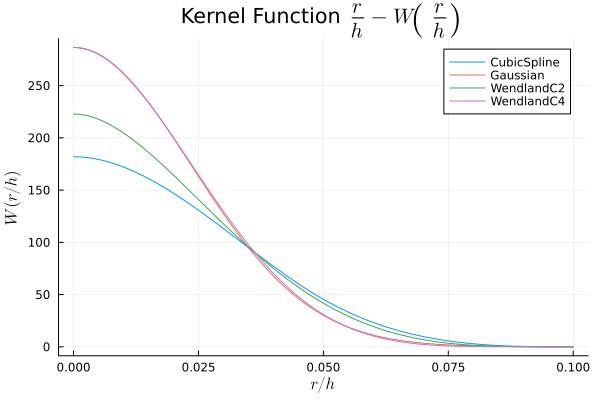
\includegraphics[width=0.9\textwidth]{images/kernel_value.png}
        \caption{光滑核函数的值}
    \end{figure}
\end{frame}

\begin{frame}
    记 $q=\frac{r}{h}$,则 $\vec{\nabla} W$ 的表达式为:
    \begin{equation}
        \begin{aligned}
            \vec{\nabla} W 
            &= \vec{e}_i\frac{\partial}{\partial x_i}W\left(\frac{r}{h}\right)\\
            &= W^\prime(q)\frac{1}{h}\vec{e}_i\frac{\partial r}{\partial x_i}\\
            &= \frac{1}{h}W^\prime(q) \frac{x_i}{r}\vec{e}_i\\
        \end{aligned}
    \end{equation}
    其中 $W^\prime(q)$ 为光滑核函数关于相对半径 $q$ 的导数。
    可以发现光滑核函数的梯度与 $x_i\vec{e}_i$ 有着一致的方向,且:
    \begin{equation}
        |\vec{\nabla}W| = \left|\frac{1}{h}W^\prime(q)\right|
    \end{equation}
\end{frame}

\begin{frame}
    如下图为目前实现的四个光滑核函数的 $\frac{1}{h}W^\prime(q)$ 在光滑核半径为 $0.1$ 时的值。
    可以发现 $W^\prime(q)$ 恒负,该结果我和开源库比较过,是一致的。
    \begin{figure}[H]
        \centering
        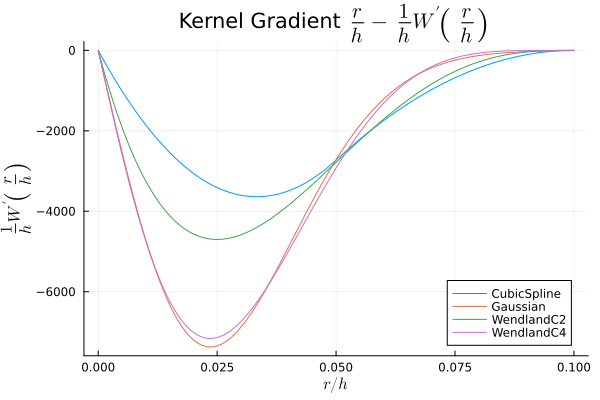
\includegraphics[width=0.9\textwidth]{images/kernel_gradient.png}
        \caption{光滑核函数的梯度值}
    \end{figure}
\end{frame}

\subsection{SPH 方法的基本方程}

\begin{frame}
    在 Lagrange 描述下,不可压流体的基本方程为,
    暂时不考虑能量方程。
    \begin{equation}
        \begin{aligned}
            \frac{\mathrm{d} \rho}{\mathrm{d} t} &= -\rho \nabla \cdot \vec{v} \\
            \frac{\mathrm{d} \vec{v}}{\mathrm{d} t} &= -\frac{1}{\rho} \nabla p + \vec{g} + \nu \nabla^2 \vec{v}\\
            \frac{\mathrm{d} \vec{x}}{\mathrm{d} t} &= \vec{v}
        \end{aligned}
    \end{equation}
    目前 SPH 方法广为使用的方式是弱可压 WCSPH 方法,
    其允许流体的密度在一定范围内变化。
    并且给出了状态方程如下:
    \begin{equation}
        p = \frac{c_0^2\rho_0}{\gamma}
        \left[\left(\frac{\rho}{\rho_0}\right)^\gamma - 1\right]=
        \frac{c_0^2\rho_0}{\gamma}
        \left[\left(1+\frac{\rho-\rho_0}{\rho_0}\right)^\gamma - 1\right]
    \end{equation}
    在 $\rho$ 变化不大时,方程可以退化为 $p=c_0^2(\rho-\rho_0)$。
\end{frame}

\begin{frame}
    对于上述方程,
    我查阅了一些开源库和书籍论文,
    他们对于 $c_0$ 这个量的设定是“人工声速”。
    并非是真正的水的声速。
    而 $\gamma$ 一般设定为 $7$。
    可以推导在这种状态方程下,
    声速为:
    \begin{equation}
        c^2=\frac{\partial p}{\partial \rho}=c_0^2\left(\frac{\rho}{\rho_0}\right)^{\gamma - 1}
    \end{equation}
    而 $c_0$ 的值需要根据不同的算例设定不同的值来保证程序稳定性,
    一般取为:
    \begin{equation}
        c_0 = 10\max \{U_{\max}, \sqrt{g L_{\max}}\}
    \end{equation}
    这里的人工声速选取是我在程序内头痛的一个事情,我会在后续叙述。
\end{frame}

\subsection{SPH 方法的数值离散}

\begin{frame}
    根据光滑核函数插值,
    我们可以将 SPH 的控制方程离散成光滑核函数的插值形式:
    \begin{equation}
        \begin{aligned}
            \frac{\mathrm{d} \rho_i}{\mathrm{d} t} &= \rho_i \sum_j m_j \vec{v}_{ij} \cdot \nabla W_{ij} \\
            \frac{\mathrm{d} \vec{v}_i}{\mathrm{d} t} &= -\sum_j m_j \left(\frac{p_i}{\rho_i^2} + \frac{p_j}{\rho_j^2}\right) \nabla W_{ij} + \vec{g} + \nu \nabla^2 \vec{v}_i
        \end{aligned}
    \end{equation}
    其中粘性项的离散形式我没数学能力推导,
    直接采用了 SPHysics 开源库给出的形式如下:
    \begin{equation}
        \nu \nabla^2 \vec{v}_i = 
        \sum_j m_j
        \frac{4 (\mu_i + \mu_j) \vec{r}_{ij}\cdot \nabla W_{ij}}{(\rho_i + \rho_j)^2 (r_{ij}^2 + 0.01h^2)}\vec{v}_{ij}
    \end{equation}
\end{frame}
\section{近一个月的工作与内容新增}

\subsection{程序的重构}

\begin{frame}
    \frametitle{\subsecname}
    \begin{itemize}
        \item 为了方便 debug 和后续的功能扩展,我对程序进行了重构。
        用 Julia 重写了一下。
        首先 Julia 是基于 MIT 协议的,可以闭源商用。
        \item 速度接近于 C ,一般认为优化合理的情况下仅有 5\% 的性能损失。
        我目前手中有一份 C++ 和一份 Julia 的代码,
        在我使用过程中感觉速度上没有太大的差别。
        \item 当然如果后续确定需要做这个方向,
        并且课题组不满意 Julia 的开发版本的话,
        我可以在其基础上用 C++ 重写一份。
        \item 引入 Julia 的目的有四个:
        \begin{itemize}
            \item 动态的实现邻域粒子搜索功能;
            \item 用上锁的方法实现了简单的多线程并行计算;
            \item 用多重派发实现了对不同粒子行为定义
            \item 方便做单步测试和后处理,这点比 C++ 好很多。
        \end{itemize}
    \end{itemize}
\end{frame}

\subsection{XSPH 方法的引入}

\begin{frame}
    \frametitle{\subsecname}
    \begin{itemize}
        \item 为了解决 SPH 方法的数值耗散问题,Monaghan 在 1992 年提出了 XSPH 方法。
        \item XSPH 方法的思想是在粒子的速度上加上一个由粒子间相对位置计算得到的修正项。
        \item 该修正项的计算公式为:
        \begin{equation}
            \tilde{v}_i = v_i - \epsilon \sum_j m_j \frac{2\vec{v}_{ij}}{\rho_i+\rho_j} W_{ij}
        \end{equation}
        据文献中介绍,$\epsilon$ 的取值范围为 $0\sim 1$。
        不过上式仅在计算粒子的位置时使用,计算粒子的速度时仍然使用原来的速度。
        根据 SPHysics 和 Monaghan 本人介绍,该方法让粒子移动更趋于平整。
    \end{itemize}
\end{frame}

\subsection{物理场的核函数重构}

\begin{frame}
    \frametitle{\subsecname}
    对于存在自由表面的流体,因其物理粒子在周边的缺失,
    会导致物理量的计算出现较大误差。
    尤其是对于密度场需要进行核函数的修正。
    \begin{figure}[H]
        \centering
        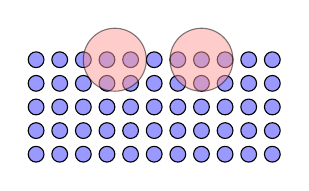
\begin{tikzpicture}
            % several particles
            % 4 row, 5 column
            \foreach \x in {0,1,2,3,4,5,6,7,8,9,10}
            \foreach \y in {0,1,2,3,4}
            \filldraw[fill=blue!40!white, draw=black] (0.3*\x,0.3*\y) circle (0.1);
            % draw a circle at the top row in the middle, alpha = 0.5
            \draw[fill=red!40!white, draw=black, opacity=0.5] (1.0,1.2) circle (0.4);
            % draw a circle at the top row in the middle, alpha = 0.5
            \draw[fill=red!40!white, draw=black, opacity=0.5] (2.1,1.2) circle (0.4);
        \end{tikzpicture}
    \end{figure}
    \begin{equation}
        \hat{\rho}_i = \frac{
            \sum_j m_j W_{ij}
        }{
            \sum_j \frac{m_j}{\rho_j}W_{ij}
        }
    \end{equation}
    据 SPHysics 中介绍,该修正方法可以有效地减小自由表面附近的误差。
    该步骤无需每步迭代都进行,一般每 10 步进行一次即可。
    也有推荐值 30 步一次。
    并且该核函数修正法也可以用于其他物理量的修正。
\end{frame}

\subsection{邻域搜索}

\begin{frame}
    \frametitle{\subsecname}
    因为 Lagrange 描述法中,每个粒子的所在位置是随时间变化的,
    所以需要在每一步迭代中都对每个粒子的光滑核半径内的邻域(支撑域)进行搜索。
    正常的实现每步都是复杂度为 $O(N^2)$ 的算法。

    一个较为直接的优化方法是将空间划分为背景网格,
    将每个粒子所在的网格单元的周围 9 个(二维)或 27 个(三维)单元的粒子都加入到该粒子的邻域搜索中。
    这样可以将搜索复杂度降低到 $O(N\log N)$。

    \begin{figure}[H]
        \centering
        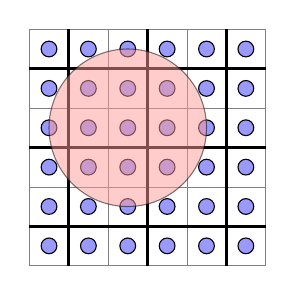
\begin{tikzpicture}
            % draw the background
            \draw[step=0.5cm,gray,very thin] (-1.5,-1.5) grid (1.5,1.5);
            % draw the main grid
            \draw[step=1cm,black,very thick] (-1.5,-1.5) grid (1.5,1.5);
            % draw the particles
            % random position
            \foreach \x in {-1.25,-0.75,...,1.25}
            \foreach \y in {-1.25,-0.75,...,1.25}
            \filldraw[fill=blue!40!white, draw=black] (\x,\y) circle (0.1);
            % draw the circle
            \draw[fill=red!40!white, draw=black, opacity=0.5] (-0.25,0.25) circle (1);
        \end{tikzpicture}
    \end{figure}
    这需要高级的数据结构的,
    自己手写的安全性和效率未必高。
    目前用了 MIT 协议的三方库,如果要自己实现需要 HashMap 和 KD-Tree。
\end{frame}

\subsection{固壁边界条件的实现}

\begin{frame}
    \frametitle{\subsecname}
    在查询了 SPHysics 的源代码以及一本河海大学老师写的书之后,
    我发现他们都采用了一种“虚拟粒子”的方法来实现固壁边界条件。
    \begin{figure}[H]
        \centering
        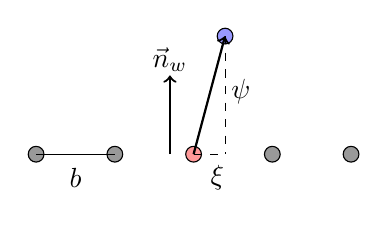
\begin{tikzpicture}
            \foreach \x in {0,1,3,4}
            \draw[fill=black!40!white, draw=black] (\x,0) circle (0.1);
            \draw[fill=blue!40!white, draw=black] (2.4,1.5) circle (0.1);
            \draw[fill=red!40!white, draw=black] (2,0) circle (0.1);
            
            \draw[->, thick] (2,0) -- (2.4,1.5);
            \draw[->, thick] (1.7,0) -- (1.7,1);
            \node at (1.7,1.2) {$\vec{n}_w$};
            \draw[dashed] (2.4,1.5) -- (2.4,0);
            \draw[dashed] (2, 0) -- (2.4,0);

            \draw[-] (0,0)--(1,0);
            \node at (0.5, -0.3) {$b$};

            \node at (2.6,0.8) {$\psi$};
            \node at (2.3, -0.3) {$\xi$};
        \end{tikzpicture}
    \end{figure}
    \begin{equation}
        \vec{f}_w=P(\psi)R(\xi)\epsilon(u_{\perp},z)\vec{n}_w
    \end{equation}
    $\psi$ 为粒子到壁面的距离,$\xi$ 为粒子到壁面粒子投影的距离,
    $u_{\perp}$ 为粒子在壁面法向的速度,$z$ 为粒子的水中深度,
    $\vec{n}_w$ 为壁面法向单位向量。
\end{frame}

\begin{frame}
    \frametitle{\subsecname}
    其中 $P(\xi)$ 计算公式如下:
    \begin{equation}
        P(\xi)=A\frac{1}{\sqrt{q}}(1-q)
    \end{equation}
    其中:
    \begin{equation}
        q=\frac{\psi}{2h}\quad A = 0.01\frac{1}{h}c_i^2
    \end{equation}
    事实上这里的壁面虚拟力的设置会发现极大,
    之前程序中 $\frac{1}{h}$ 忘了除发现可以正常算出来,
    但是除了以后发现程序反而容易炸(靠 bug 运行?)。
    $R(\xi)$ 的计算公式如下,是一个沿壁面周期性变化的函数:
    \begin{equation}
        R(\xi)=\frac{1}{2}\left[
            1+\cos\left(\frac{2\pi\xi}{b}\right)
        \right]
    \end{equation}
\end{frame}

\begin{frame}
    \frametitle{\subsecname}
    $\epsilon(u_{\perp},z)$ 的计算公式分为两部分:
    \begin{equation}
        \epsilon(u_{\perp},z)=\epsilon (u_{\perp})+\epsilon(z)
    \end{equation}
    其中:
    \begin{equation}
        \epsilon(u_{\perp})=
        \begin{cases}
            0 &\quad u_{\perp}\geq 0\\
            -\frac{20u_{\perp}}{c_0} &\quad -20u_{\perp}<c_0\\
            1 &\quad -20u_{\perp}\geq c_0
        \end{cases}
    \end{equation}
    \begin{equation}
        \epsilon(z)=
        \begin{cases}
            0 &\quad z\geq 0\\
            -\frac{z}{h_0} &\quad -h_0<z<0\\
            1 &\quad -h_0\geq z
        \end{cases}
    \end{equation}
    其中 $c_0$ 为声速,$h_0$ 为参考水深。
    这一项可以看出这两项是对粒子的移动速度和压力深度作了修正。
    靠近壁面速度大、压力深度大的粒子受到壁面的作用力也更大。
\end{frame}

\begin{frame}
    \frametitle{\subsecname}
    这里有一个问题,就在于这个壁面虚拟力的计算公式中,$A$ 这一项。
    我们考虑 $c_0=k\sqrt{gL}$,其中初始情况下,
    $L$ 为水的初始深度,$k$ 为一个常数一般取为 $10$。
    对于光滑核半径 $h$ 而言,总水深表示为 $L=nh$ 。
    这样的话,对于密度不大的情形,
    $A$ 这一项的数量级大约在:
    \begin{equation}
        A\sim 0.01\frac{1}{h}c_i^2\sim 0.01\frac{1}{h}k^2gL
        \sim 0.01\frac{1}{h}k^2gnh\sim 0.1k^2n
    \end{equation}
    这件事情就很奇怪,壁面力并不依赖于光滑核半径,
    而却依赖于水粒子的数量——也就是说为了匹配计算量级,
    用来离散计算域的粒子数量并不是越多越好,
    否则会导致壁面力过大。
    这边还需要再查和测试。
    \begin{figure}[H]
        \centering
        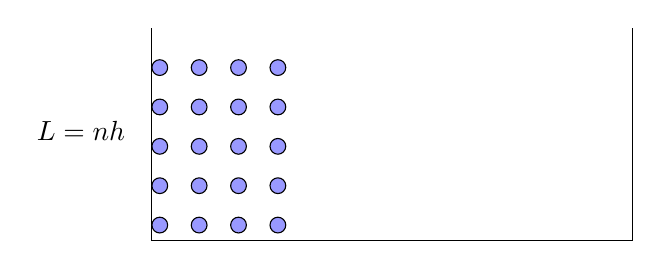
\begin{tikzpicture}
            \foreach \x in {0,1,2,3}
            \foreach \y in {0,1,2,3,4}
            \draw[fill=blue!40!white, draw=black] (0.5*\x,0.5*\y) circle (0.1);
            \draw[-] (-0.1,2.5)--(-0.1,-0.2)--(6,-0.2)--(6,2.5);
            \node at (-1,1.2) {$L=nh$};
        \end{tikzpicture}
    \end{figure}
\end{frame}

\subsection{CFL 数的文献支撑}

\begin{frame}
    \frametitle{\subsecname}
    经查询,CFL 数的计算公式与光滑核半径与人工声速有关,
    一般可以取为:
    \begin{equation}
        \Delta t = 0.1\frac{h}{c_0}
    \end{equation}
    当然上述公式的取法相当保守,
    为了加快计算速度,可以取为:
    \begin{equation}
        \Delta t = 0.1\frac{h}{V_{\max}}
    \end{equation}
    而人工声速至少是粒子速度的 10 倍,
    至此 $\Delta t,c_0,h,n_{\text{fluid}}$ 这几个参数已经耦合起来。
    当 $n_\text{fliuid}$ 较大(仿真分辨率提高)时,
    如前所述人工声速也会很大,
    这样边界力会异常大,产生数值不稳定。
    同时,如果缩小光滑核半径以缩小仿真的问题尺度,
    那么仿真时间步长也会变小,仿真时间会变长。
    这给我的程序 debug 造成了比较大的困扰。
\end{frame}

\subsection{多线程并行计算}

\begin{frame}
    \frametitle{\subsecname}
    为了提高程序的运行效率,我引入了多线程并行计算。
    这里先简单运用了线程锁的方式对程序进行了简单的并行计算。
    不过从计算效率来看,
    上锁的并行方式对并行效率是有影响的。
    对比与之前串行、未进行邻域搜索的 C++ 程序而言计算效率大概如下表所示:
    \begin{table}[H]
        \centering
        \begin{tabular}{c|c|c}
            \hline
            1800粒子 & $h/dr=1.5$ & $h/dr=3$ \\
            \hline
            C++ & 8it/s & 7it/s \\
            Julia+邻域搜索 & 30it/s & 21it/s \\
            Julia+邻域搜索+10线程 & 108it/s & 76it/s \\
            \hline
        \end{tabular}
    \end{table}
    当然我也在反思程序结构本身是不是不太适合并行,
    可能后面上 MPI 并行和 GPU 并行的时候需要先学一下并行原理,
    再对于程序结构进行重构。
\end{frame}


\section{标准算例的对比}

\subsection{标准算例介绍}

\begin{frame}
    \frametitle{\subsecname}
    \begin{figure}[H]
        \centering
        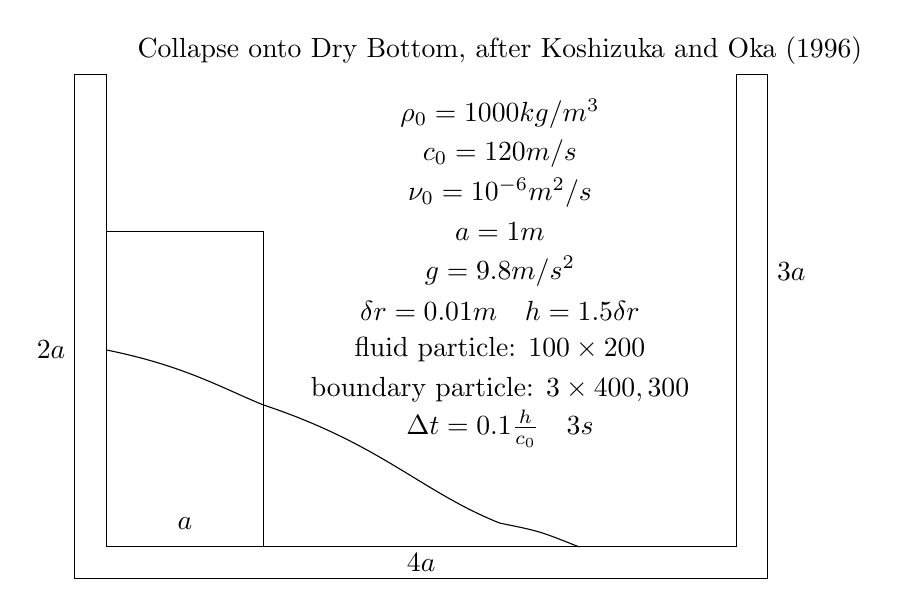
\begin{tikzpicture}
            \draw[-] (0,6)--(0,0)--(8,0)--(8,6);
            \draw[-] (0,6)--(-0.4,6)--(-0.4,-0.4)--(8.4,-0.4)--(8.4,6)--(8,6);
            \draw[-] (0,4)--(2,4)--(2,0);
            
            % arbitrary fluid surface at some time
            \draw (0,2.5) .. controls (1,2.3) and (1.5,2.0) .. (2,1.8) .. controls (3.5,1.3) and (4,0.7) .. (5,0.3) .. controls (5.5,0.2) .. (6,0);
            
            \node at (1,0.3) {$a$};
            \node at (4, -0.2) {$4a$};
            \node at (-0.7, 2.5) {$2a$};
            \node at (8.7, 3.5) {$3a$};

            \node at (5, 6.3) {Collapse onto Dry Bottom, after Koshizuka and Oka (1996)};
            \node at (5, 5.5) {$\rho_0=1000kg/m^3$};
            \node at (5, 5) {$c_0=120m/s$};
            \node at (5, 4.5) {$\nu_0=10^{-6}m^2/s$};
            \node at (5, 4) {$a=1m$};
            \node at (5, 3.5) {$g=9.8m/s^2$};
            \node at (5, 3) {$\delta r=0.01m\quad h=1.5\delta r$};
            \node at (5, 2.5) {fluid particle: $100\times 200$};
            \node at (5, 2) {boundary particle: $3\times 400,300$};
            \node at (5, 1.5) {$\Delta t=0.1\frac{h}{c_0}\quad 3s$};
        \end{tikzpicture}
    \end{figure}
\end{frame}

\subsection{踩的第一个坑:似是而非的结果}

\begin{frame}
    \frametitle{\subsecname}
    如下图,
    见 WaterWallDemo.mp4 。
    一开始我以为是对的,但再细看之下,
    发现壁面内粒子还是发生了穿透,
    只是我加的墙体粒子比较厚,未穿出。
    比如139步的右下角,就有粒子嵌入墙壁。
    \begin{figure}[H]
        \centering
        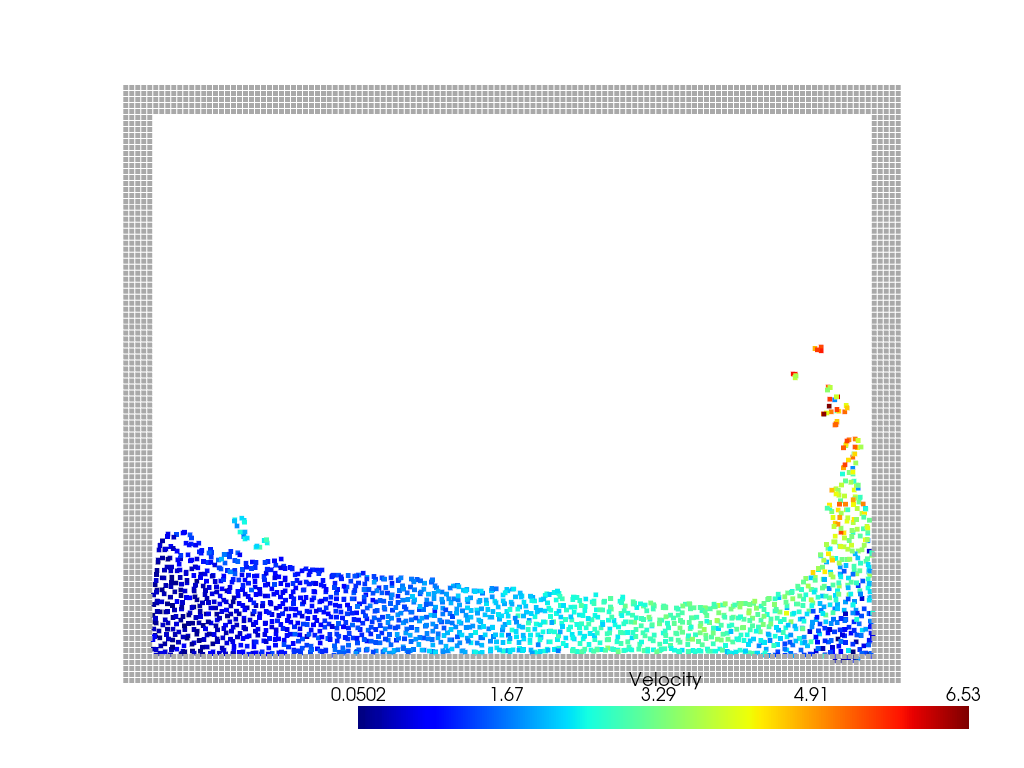
\includegraphics[width=0.7\textwidth]{images/first_trial_139.png}
    \end{figure}
\end{frame}

\subsection{踩的第二个坑:壁面的处理}

\begin{frame}
    \frametitle{\subsecname}
    然后我排查了一下程序,
    发现是在程序内壁面力没有乘 $\frac{1}{h}$ 系数。
    改完后会发现水体发生了异常的迸溅和分离,
    尤其是顶层水体像是受到了壁面异常的拍击,
    临近边界的水体有明显的异常加速,与文献不符。
    \begin{figure}[H]
        \centering
        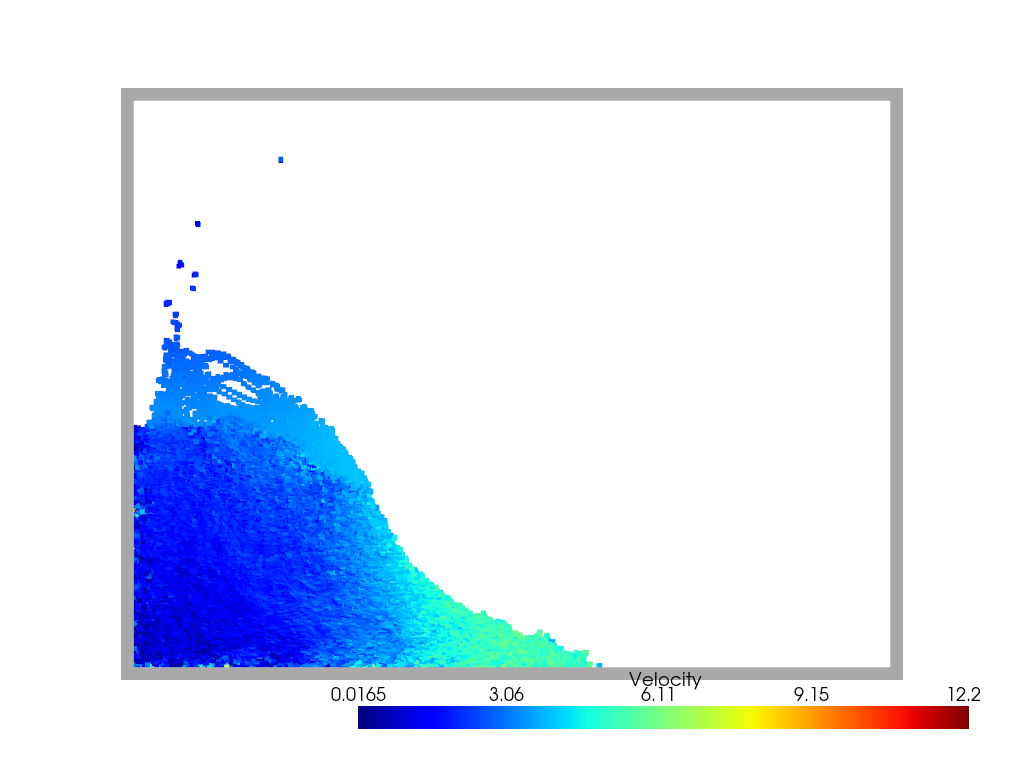
\includegraphics[width=0.7\textwidth]{images/second_trial_316.png}
    \end{figure}
\end{frame}

\begin{frame}
    \frametitle{\subsecname}
    于是我回过去推导壁面力计算公式,
    就推导出了壁面力 $f\sim 0.1k^2 n$ 的结论,
    于是怀疑可能是计算尺度的问题,
    离散化粒子太多可反而会导致计算结果不准确。
    debug 了将近一周,试了很多 $c$ 和 $h$ 以及 $dt$ 的组合。
    一无所获,程序结构还被改得很乱。
    不过这周一在看云图的过程中,
    我发现一个有趣的现象,
    下面是两张初始情况下的压强云图:
    \begin{figure}[H]
        \centering
        \subfigure[step 4]{
            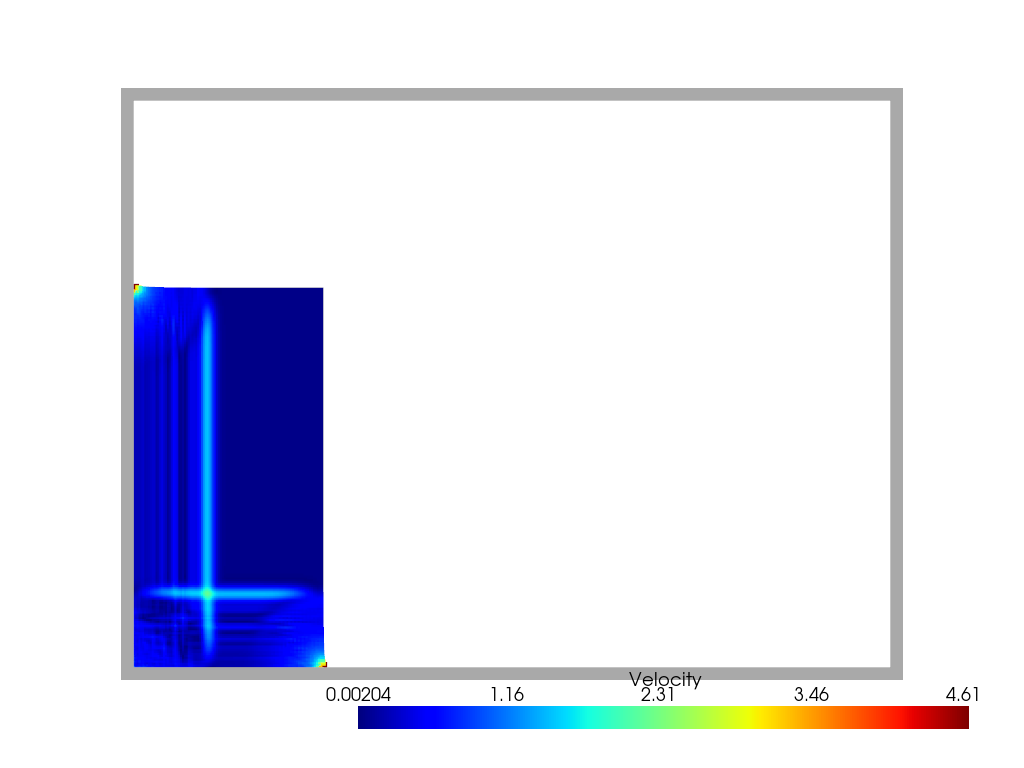
\includegraphics[width=0.45\textwidth]{images/second_trial_4.png}
        }
        \subfigure[step 6]{
            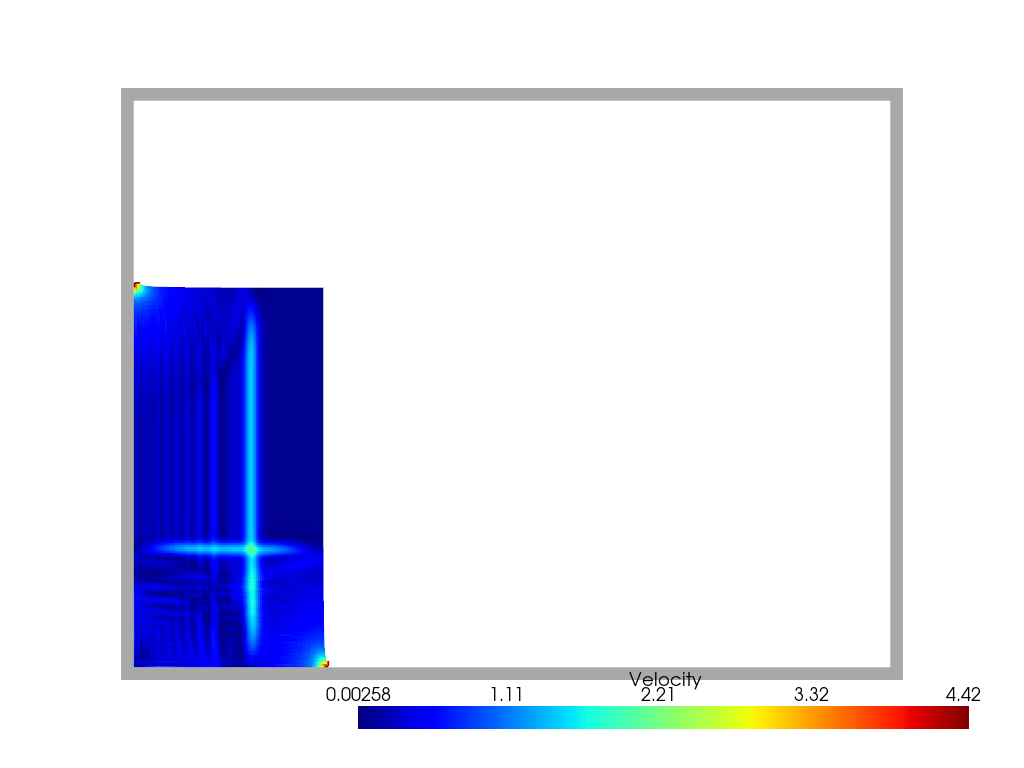
\includegraphics[width=0.45\textwidth]{images/second_trial_6.png}
        }
    \end{figure}
\end{frame}

\begin{frame}
    \frametitle{\subsecname}
    很显然的是,
    压强云图显示在初始时有一个扰动从左上角向右上角传播,
    并且同时,液体左上角开始发生崩坏,
    进而发生第一张图中的异常迸溅。
    会引起压强发生异常的水体内传播的扰动一定来源于边界力,
    于是我怀疑可能是初始时的边界给定有问题。
    \begin{figure}[H]
        \centering
        \subfigure[step 4]{
            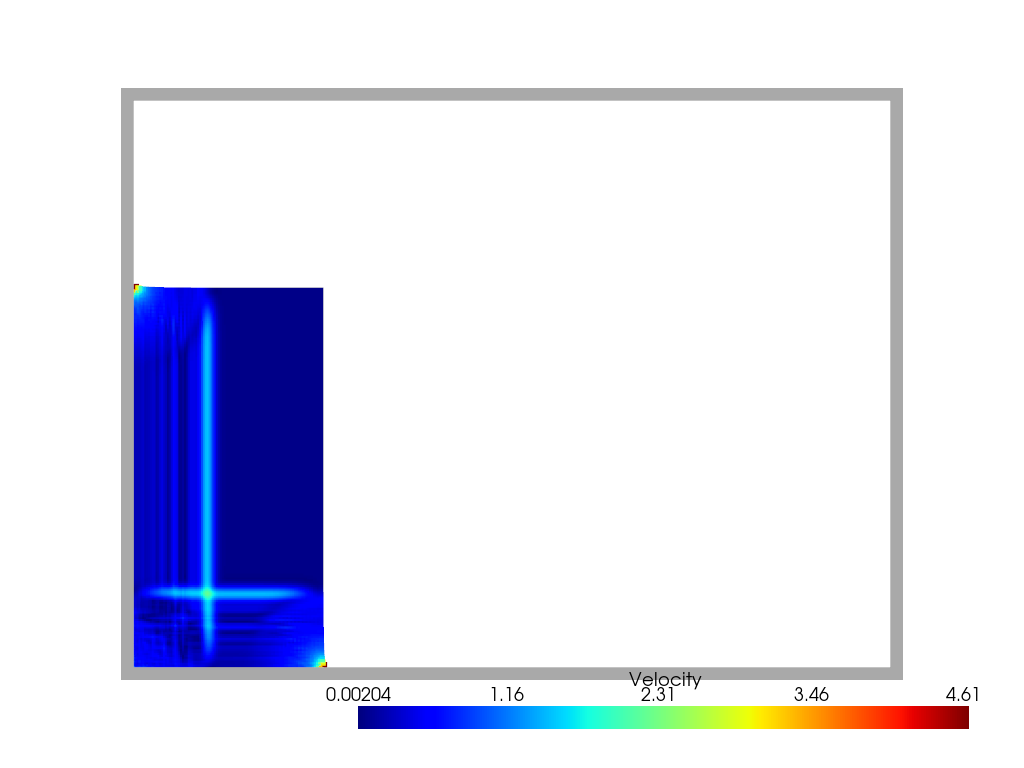
\includegraphics[width=0.45\textwidth]{images/second_trial_4.png}
        }
        \subfigure[step 6]{
            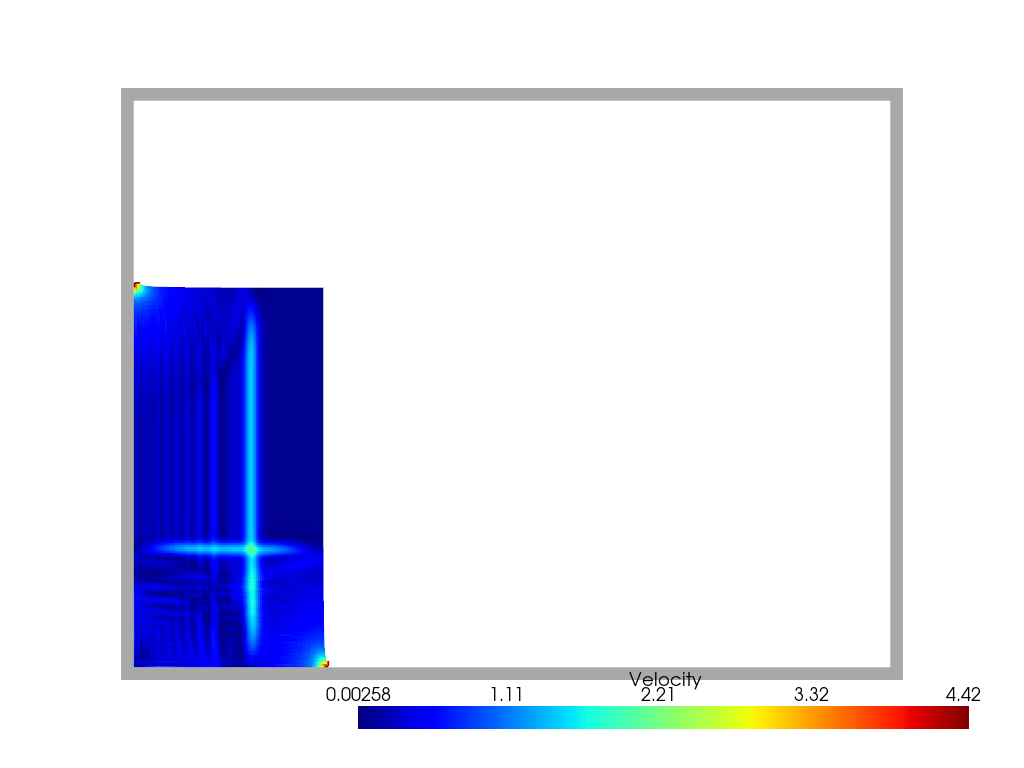
\includegraphics[width=0.45\textwidth]{images/second_trial_6.png}
        }
    \end{figure}
\end{frame}

\begin{frame}
    \frametitle{\subsecname}
    \begin{equation}
        P(\psi)=0.01\frac{1}{h}c_i^2
        \frac{1}{\sqrt{\frac{\psi}{2h}}}
        \left(1-\frac{\psi}{2h}\right)
    \end{equation}
    于是我怀疑初始边界设定不对。
    我在初始设定粒子位置时,
    是以 $dr$ 为间隔均匀分布的,
    而 $dr<h$ ,也就是初始时粒子间距小于 $h$ ,
    会有一个初始的本不该存在的初始压力项,
    而且如前所述,这项压力会给水体一个本不该存在的极大的初始扰动。
    这会让水体获得不该存在的动量,从左上角和右下角甚至水体内部崩坏。
    虽然在 SPHysics 和河海大学徐德龙教授书中公式是一致的,
    但我开始怀疑这个公式的正确性。
    \begin{figure}[H]
        \centering
        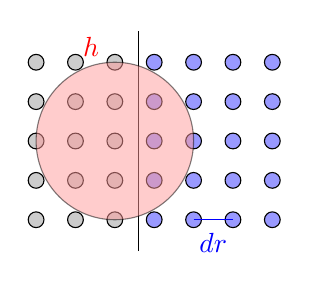
\begin{tikzpicture}
            % fluid particle
            \foreach \x in {0,1,2,3}
            \foreach \y in {0,1,2,3,4}
            \filldraw[fill=blue!40!white, draw=black] (0.5*\x,0.5*\y) circle (0.1);
            \draw[-] (-0.2,-0.4) -- (-0.2,2.4);
            % boundary particle
            \foreach \x in {-3,-2,-1}
            \foreach \y in {0,1,2,3,4}
            \filldraw[fill=gray!40!white, draw=black] (0.5*\x,0.5*\y) circle (0.1);
            
            \filldraw[fill=red!40!white, draw=black,opacity=0.5] (-0.5,0.5*2) circle (1.);

            \node[red] at (-0.8,2.2) {$h$};

            \draw[-,blue] (0.5,0) -- (1,0);
            \node[blue] at (0.75,-0.3) {$dr$};
        \end{tikzpicture}
    \end{figure}
\end{frame}

\begin{frame}
    \frametitle{\subsecname}
    鉴于 SPHysics 和徐德龙都说他们借鉴了 Rogers 在2005年的文章,
    我又去看了一下 Rogers 的文章,
    发现和 SPHysics 和徐德龙的公式完全一样,除了 $20u_{\perp}\to 40u_{\perp}$ 。
    我尝试了 Rogers 的公式,但水体崩坏的更离谱了。
    另外我还发现让 $h/dr$ 更大也会明显地让水体崩坏加剧。
    本来我以为是别的地方出了问题,
    但周二突发奇想去看了看 Rogers 引用的 Monaghan 的文章,
    发现似乎从 Rogers 开始,
    后面引用的文章全写错符号引起误解了。
    首先是沿壁面的系数 $\cos \frac{2\pi\xi}{b}$ 这项应为 $\cos \frac{\pi\xi}{b}$:
    \begin{figure}[H]
        \centering
        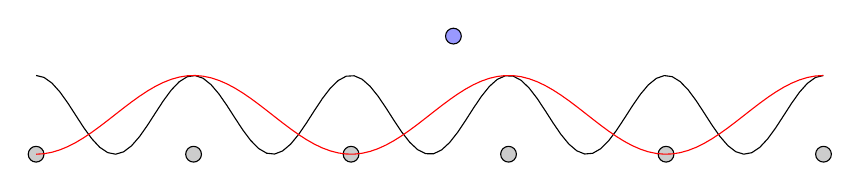
\begin{tikzpicture}
            \foreach \x in {-3,-2,-1,0,1,2}
            \filldraw[fill=gray!40!white, draw=black] (2*\x,0) circle (0.1);
            % plot cos 2pi x
            \draw[domain=-3:2,samples=100] plot (\x*2,{0.5+0.5*cos(360*\x)});
            % plot cos pi x
            \draw[domain=-3:2,samples=100,red] plot (\x*2,{0.5+0.5*cos(180*\x)});
            
            % fluid particle
            \filldraw[fill=blue!40!white, draw=black] (-0.7,1.5) circle (0.1);
        \end{tikzpicture}
    \end{figure}
\end{frame}

\begin{frame}
    \frametitle{\subsecname}
    \begin{figure}[H]
        \centering
        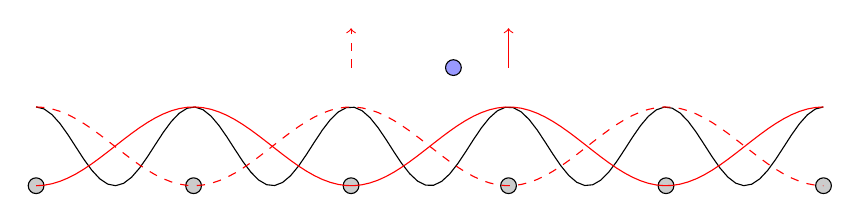
\begin{tikzpicture}
            \foreach \x in {-3,-2,-1,0,1,2}
            \filldraw[fill=gray!40!white, draw=black] (2*\x,0) circle (0.1);
            % plot cos 2pi x
            \draw[domain=-3:2,samples=100] plot (\x*2,{0.5+0.5*cos(360*\x)});
            % plot cos pi x
            \draw[domain=-3:2,samples=100,red] plot (\x*2,{0.5+0.5*cos(180*\x)});
            \draw[domain=-3:2,samples=100,red,dashed] plot (\x*2,{0.5+0.5*cos(180*(\x-1)});
            % fluid particle
            \filldraw[fill=blue!40!white, draw=black] (-0.7,1.5) circle (0.1);
            
            \draw[->,red] (0,1.5)--(0,2.0);
            \draw[->,red,dashed] (-2,1.5)--(-2,2.0);
        \end{tikzpicture}
    \end{figure}
    如上图所示,
    黑线为 $\frac{1}{2}\left(1+\cos \frac{2\pi\xi}{b}\right)$ ,
    红线为 $\frac{1}{2}\left(1+\cos \frac{\pi\xi}{b}\right)$ ,
    对于陷在两壁面粒子间的流体粒子而言,
    会受两个相邻壁面粒子的联合作用。
    对于 Monaghan 的公式,
    红色的 $\cos$ 起到叠加恒等的效果,
    而黑色的徐德龙和 Rogers 以及 SPHysics 的公式,
    在极端情况下(流体粒子在壁面粒子中间),
    两者叠加为 $0$ ,
    粒子会直接穿透壁面,不受阻碍。
\end{frame}

\begin{frame}
    \frametitle{\subsecname}
    其次是 $h$ 和 $b$ 符号的问题。
    Monaghan 原文中提到:
    where $R( y)$ is designed to fall to zero within a few particle spacings of the wall. 
    In the simulations described here, $R( y)$ is defined in terms of $q = y/(2\delta p)$ 
    (where $\delta p$ is the initial particle spacing) by the rule.
    If $q<1$ then:
    \begin{equation}
        R(y)=A\frac{1}{\sqrt{q}}(1-q)
    \end{equation}
    otherwise $R(y)=0$.
    The form of $R( y)$ is not crucial but the force must increase as $q$ decreases.
    说白了,壁面效应的作用范围不超出两倍的初始粒子间距。
    而不是光滑核半径。
    并且 $A$ 的选取也比较随意(因为这个边界叫 conpulsive boundary)。
    于是为了避免初始时的异常扰动,
    我调整了 $q/2h\to q/b$
    并进行了仿真。
    设置如前面所述,
    总共 $100\times 200$ 个流体粒子,
    $3\times (400+3+3+300\times 2)$ 个壁面粒子。
    仿真时间 $3s$ ,仿真总步数 24 万步。
\end{frame}

\subsection{目前该算例最好的计算结果以及文献对比}

\begin{frame}
    \frametitle{\subsecname}

    240.0k/240.0k [03:11:28<00:00, 21it/s]
    11489.689665 seconds (225.90 G allocations: 25.249 TiB, 17.03\% gc time, 0.03\% compilation time)

    这个程序运行了大约 11489.689665 秒(约等于 3 小时 11 分钟 28 秒),在这个过程中,它进行了大约 225.90 G(G表示十亿)次内存分配,总共分配了大约 25.249 TiB(TiB 是 Tebibyte,1 TiB 等于 1024 GiB)的内存。其中,17.03\% 的时间被用于垃圾回收(gc),0.03\% 的时间被用于编译。
    见 CollapseDry.mp4 。
\end{frame}

\begin{frame}
    \frametitle{\subsecname 0.5s}
    \begin{figure}[H]
        \centering
        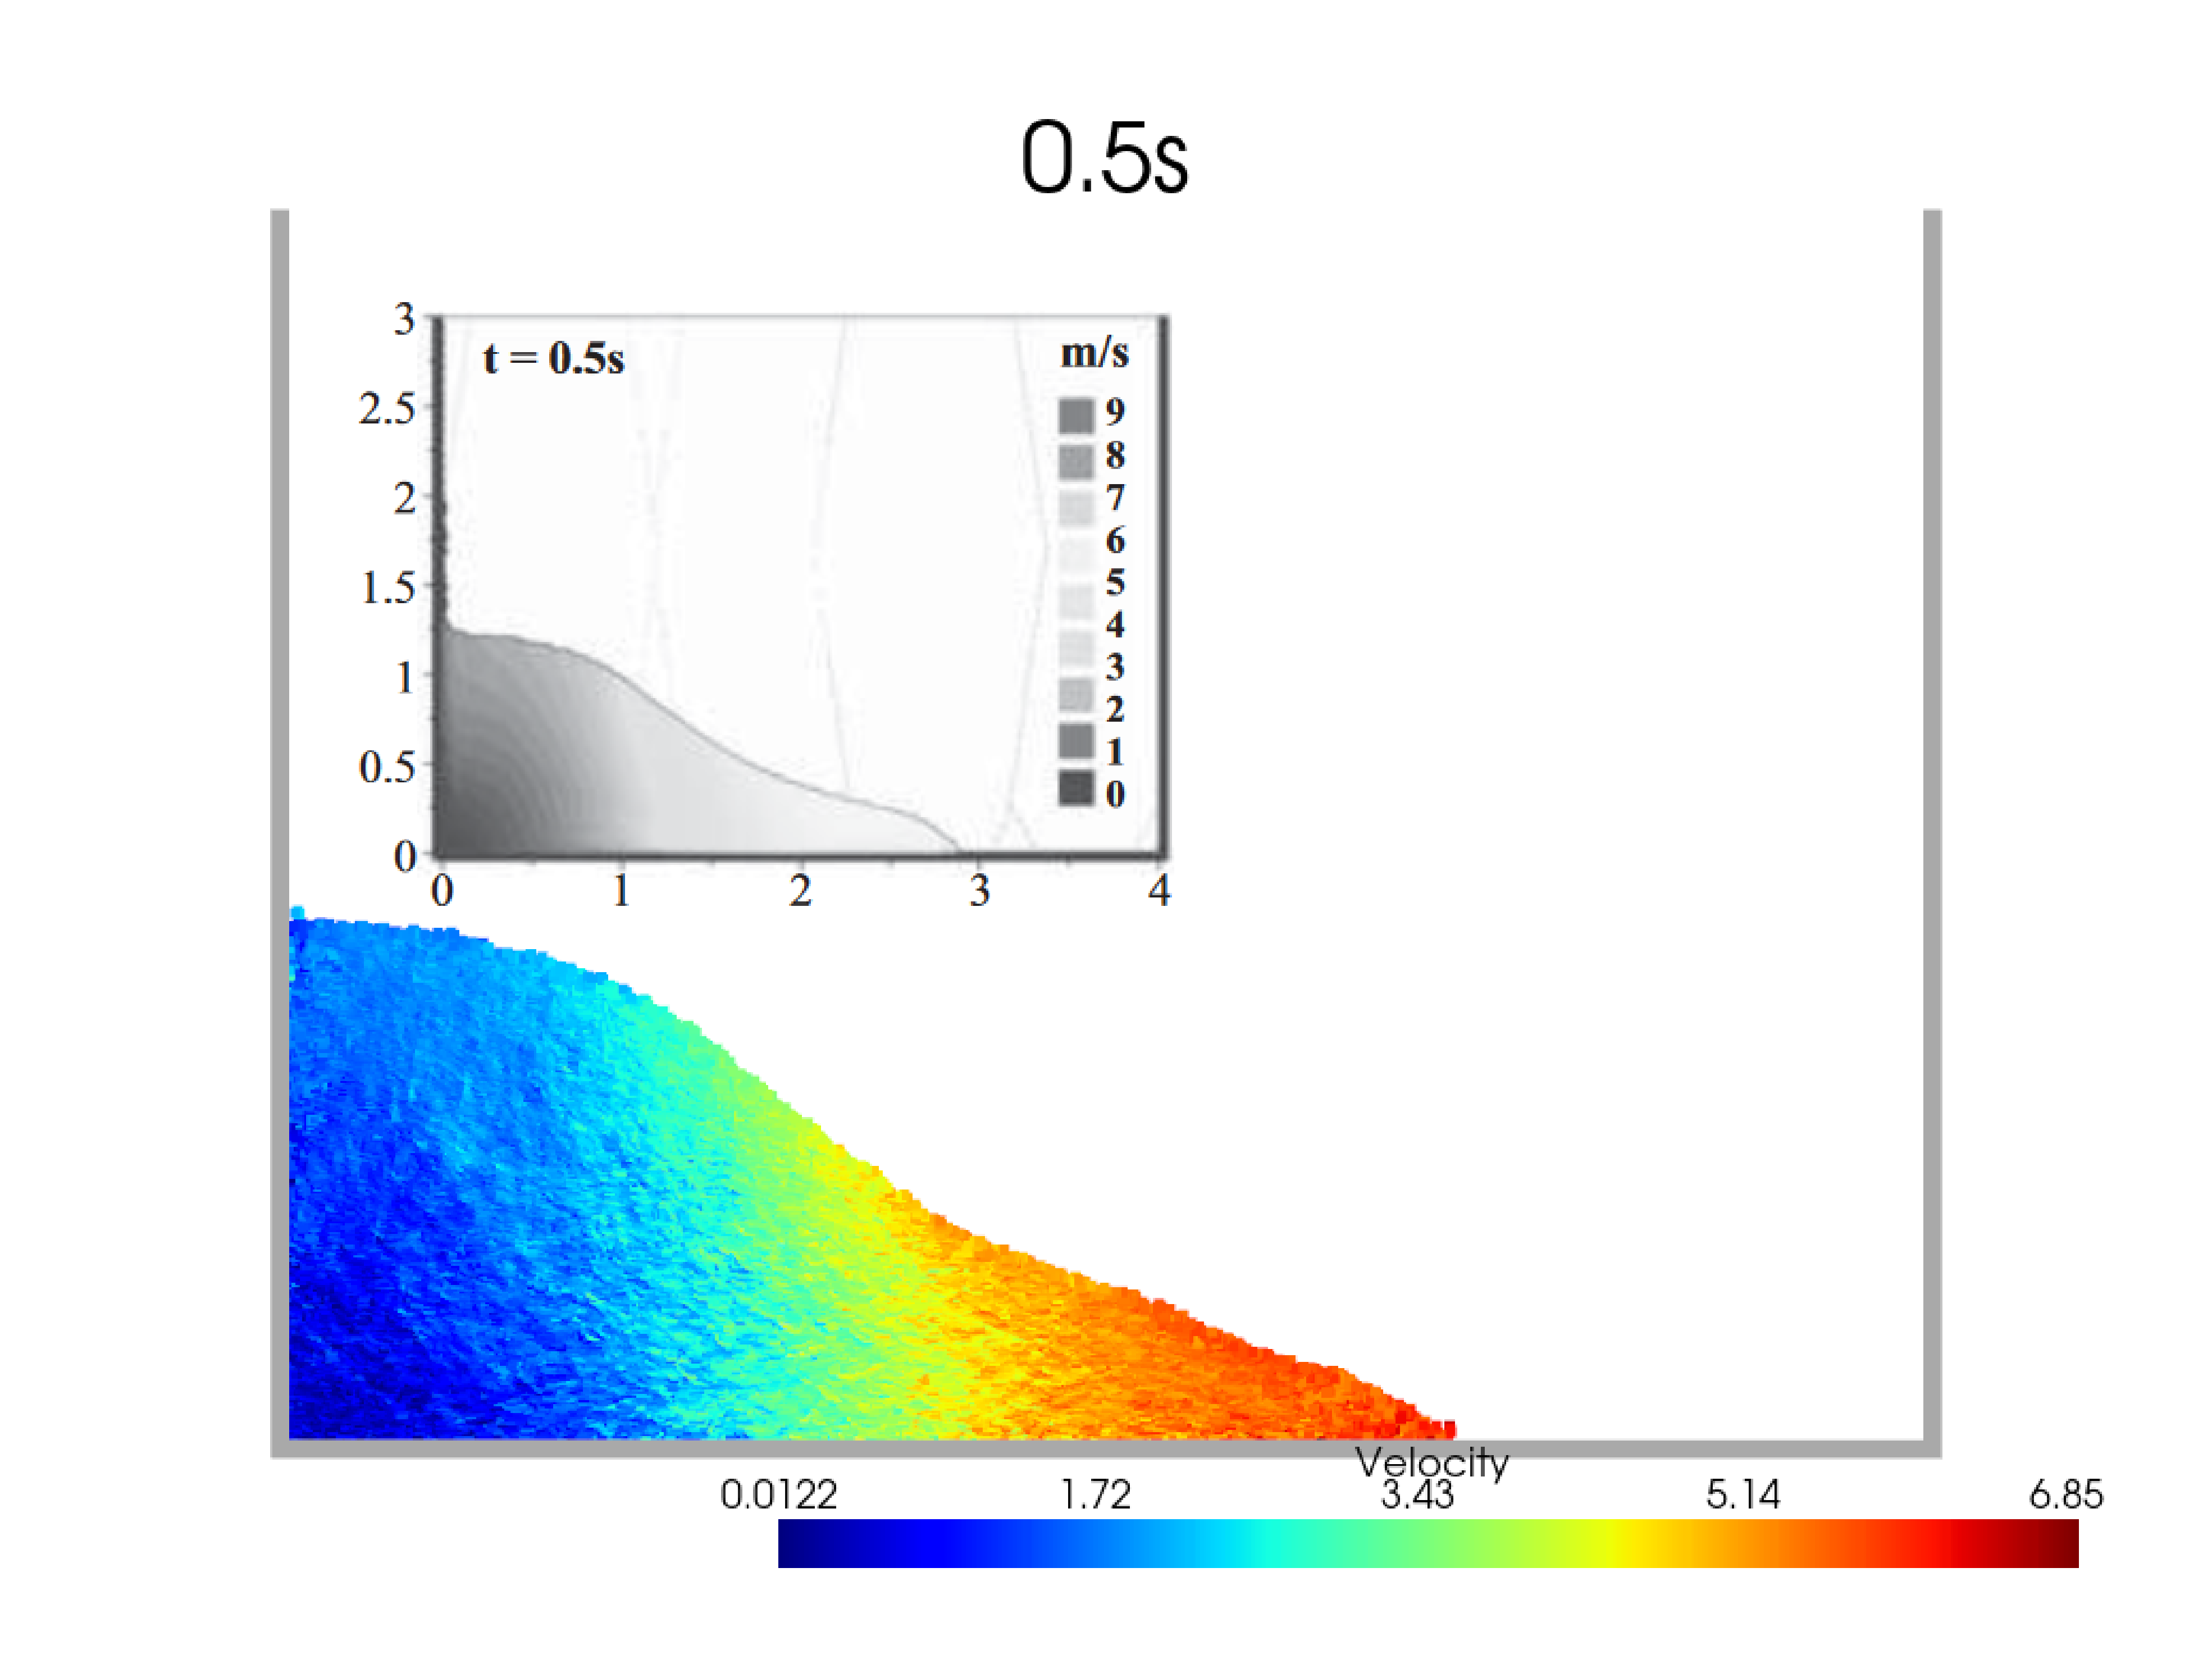
\includegraphics[width=0.9\textwidth]{images/collapse_dry05_combined.png}
    \end{figure}
\end{frame}

\begin{frame}
    \frametitle{\subsecname 1.1s}
    \begin{figure}[H]
        \centering
        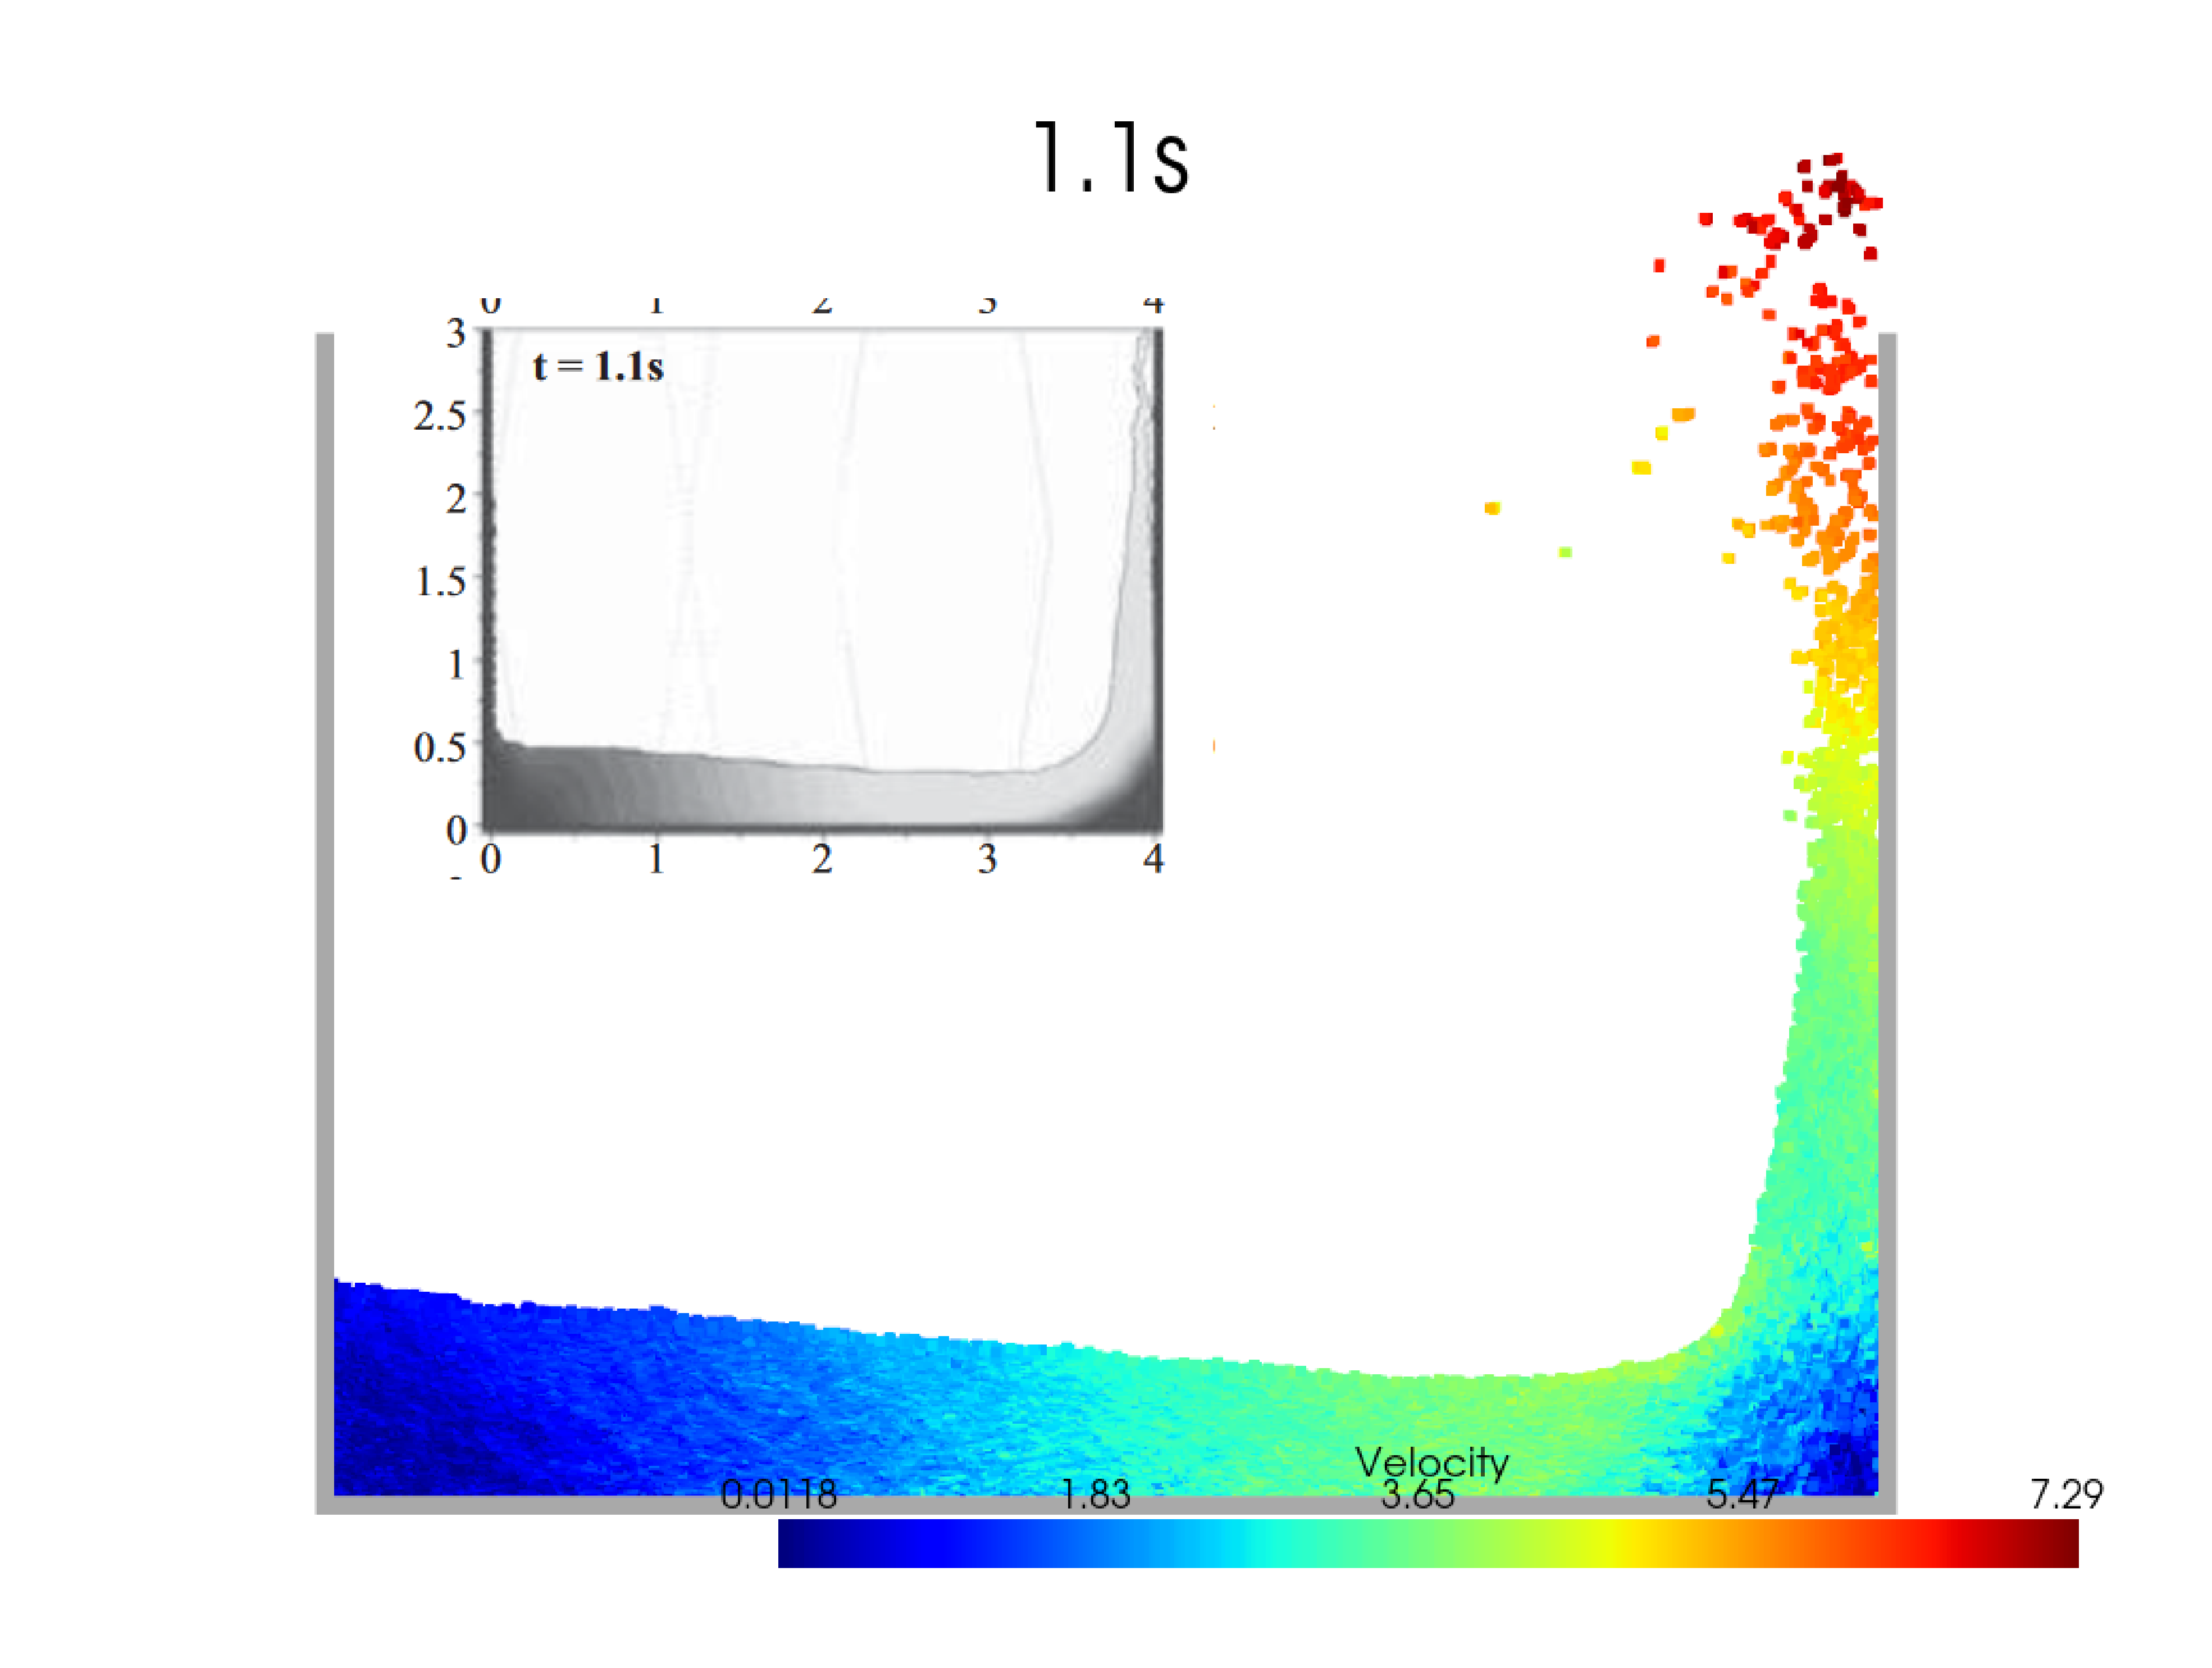
\includegraphics[width=0.9\textwidth]{images/collapse_dry11_combined.png}
    \end{figure}
\end{frame}

\begin{frame}
    \frametitle{\subsecname 1.8s}
    \begin{figure}[H]
        \centering
        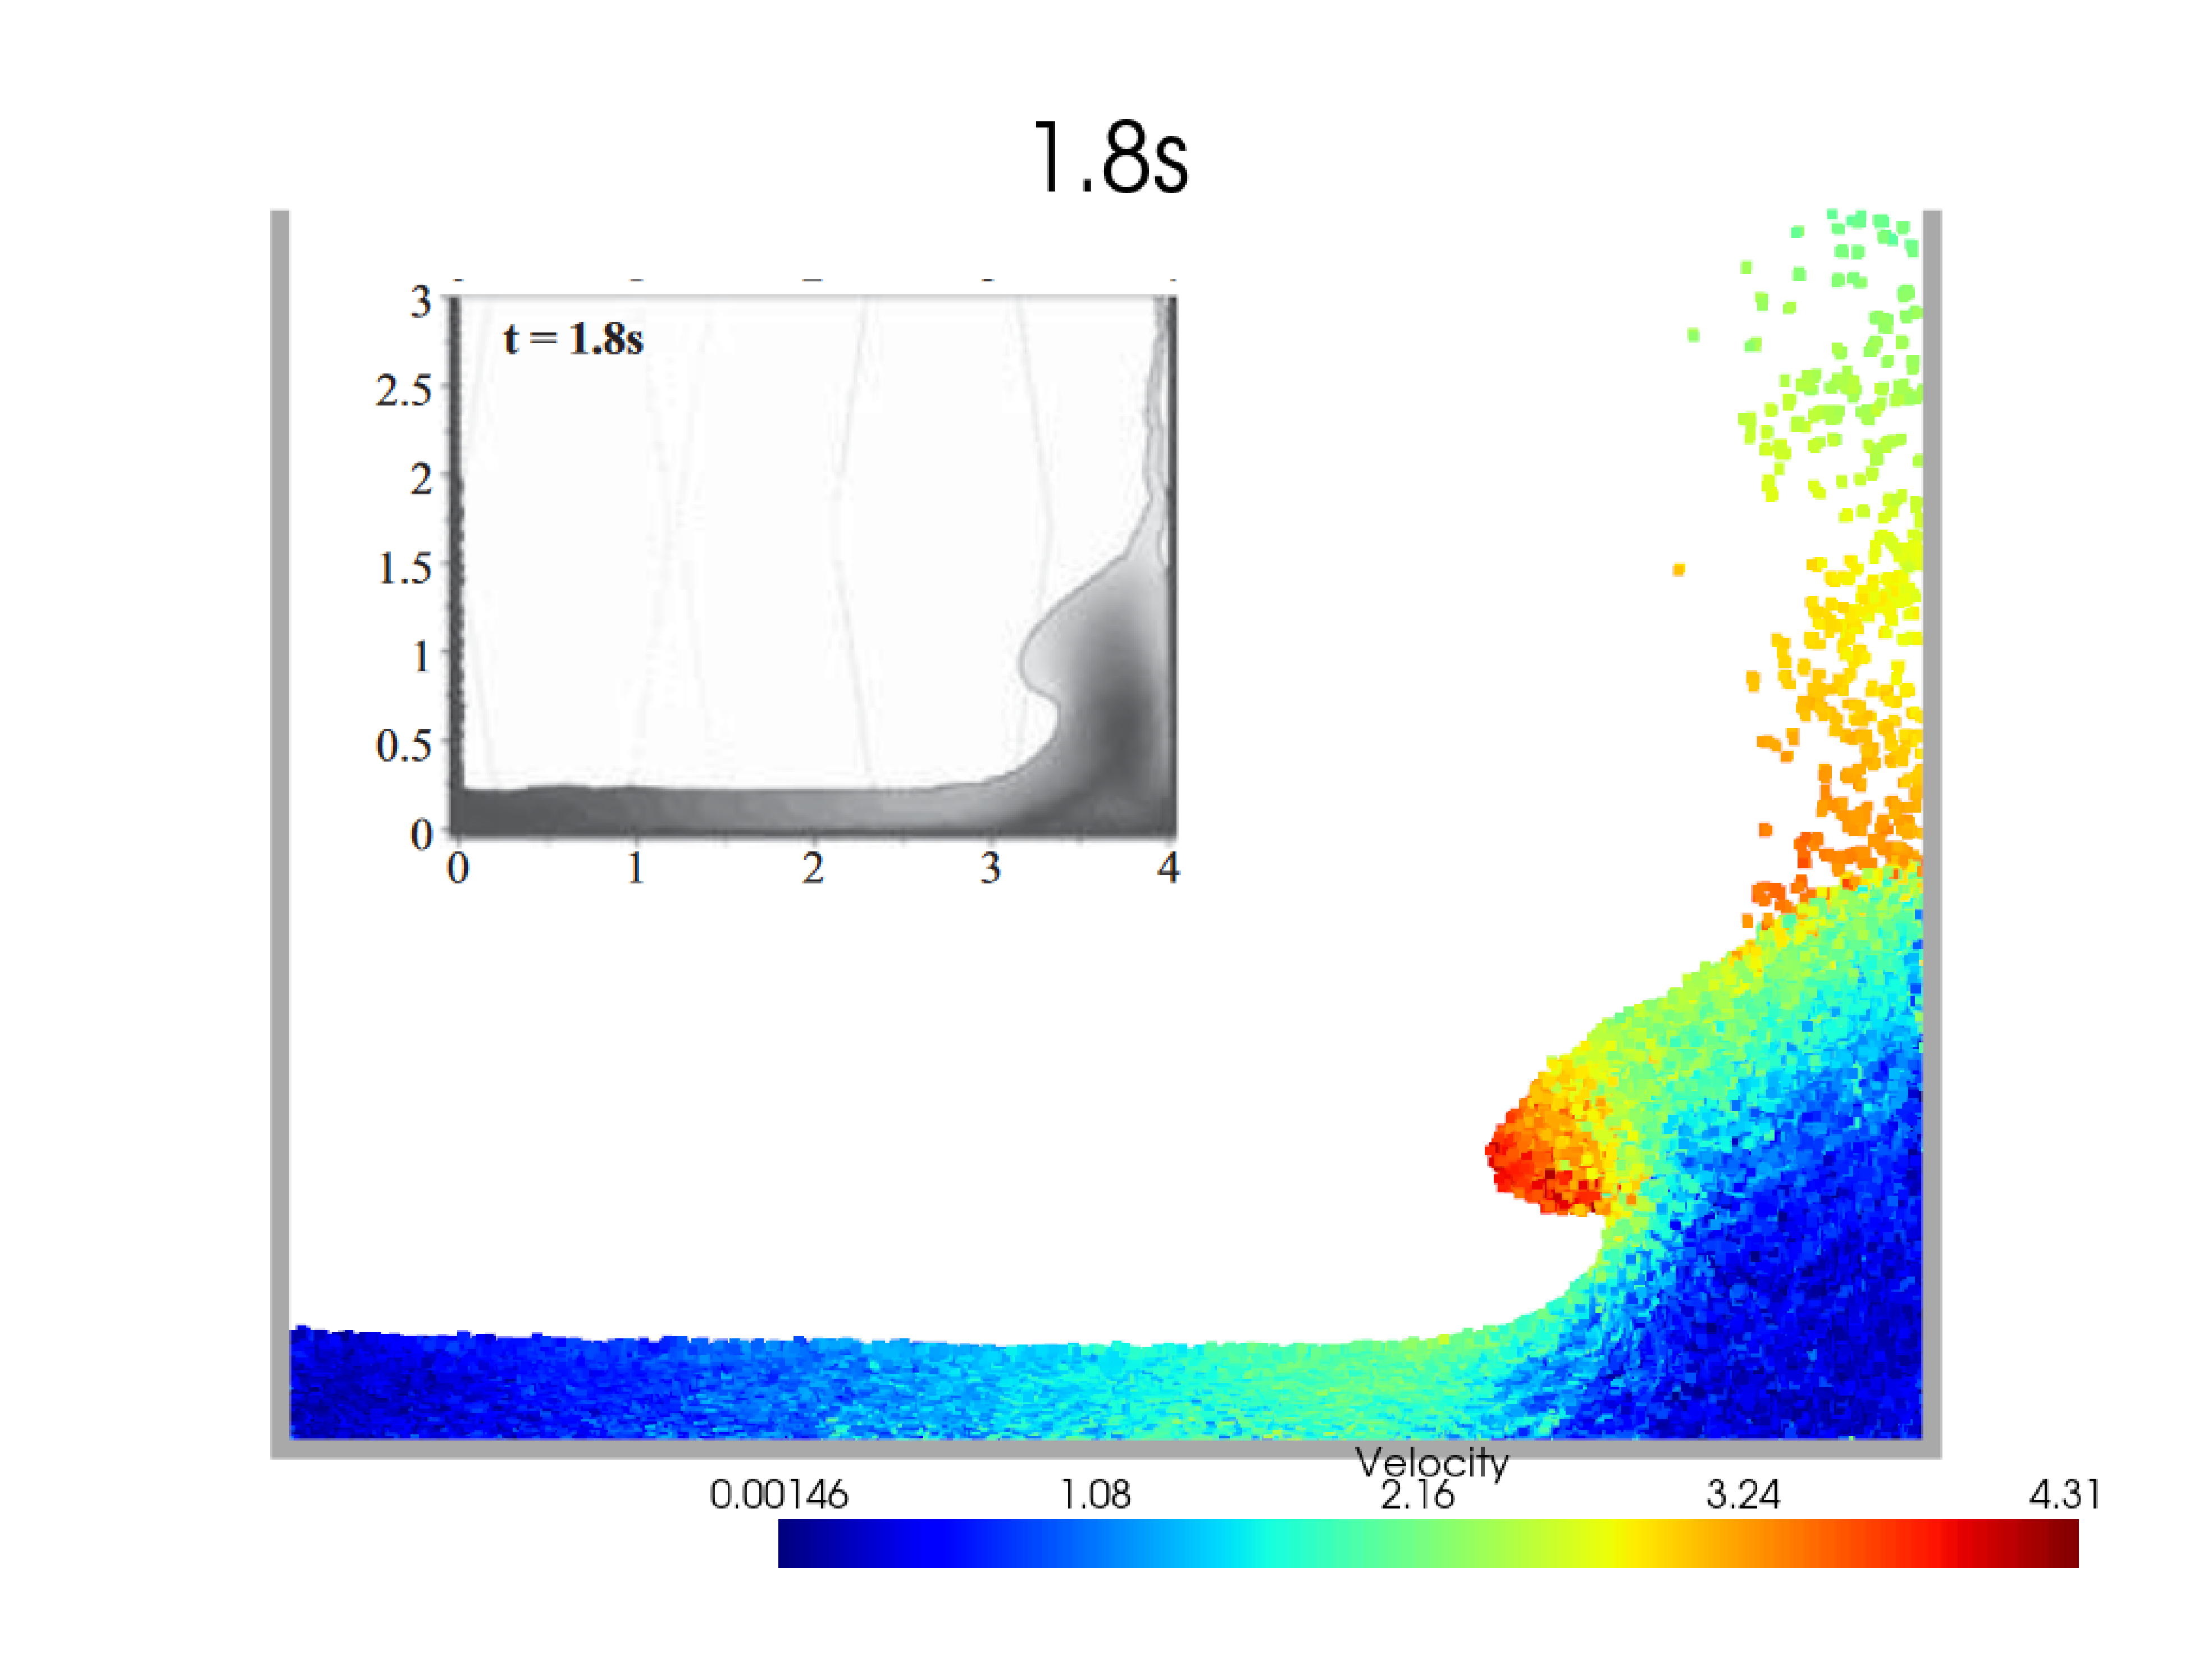
\includegraphics[width=0.9\textwidth]{images/collapse_dry18_combined.png}
    \end{figure}
\end{frame}

\begin{frame}
    \frametitle{\subsecname 2.1s}
    \begin{figure}[H]
        \centering
        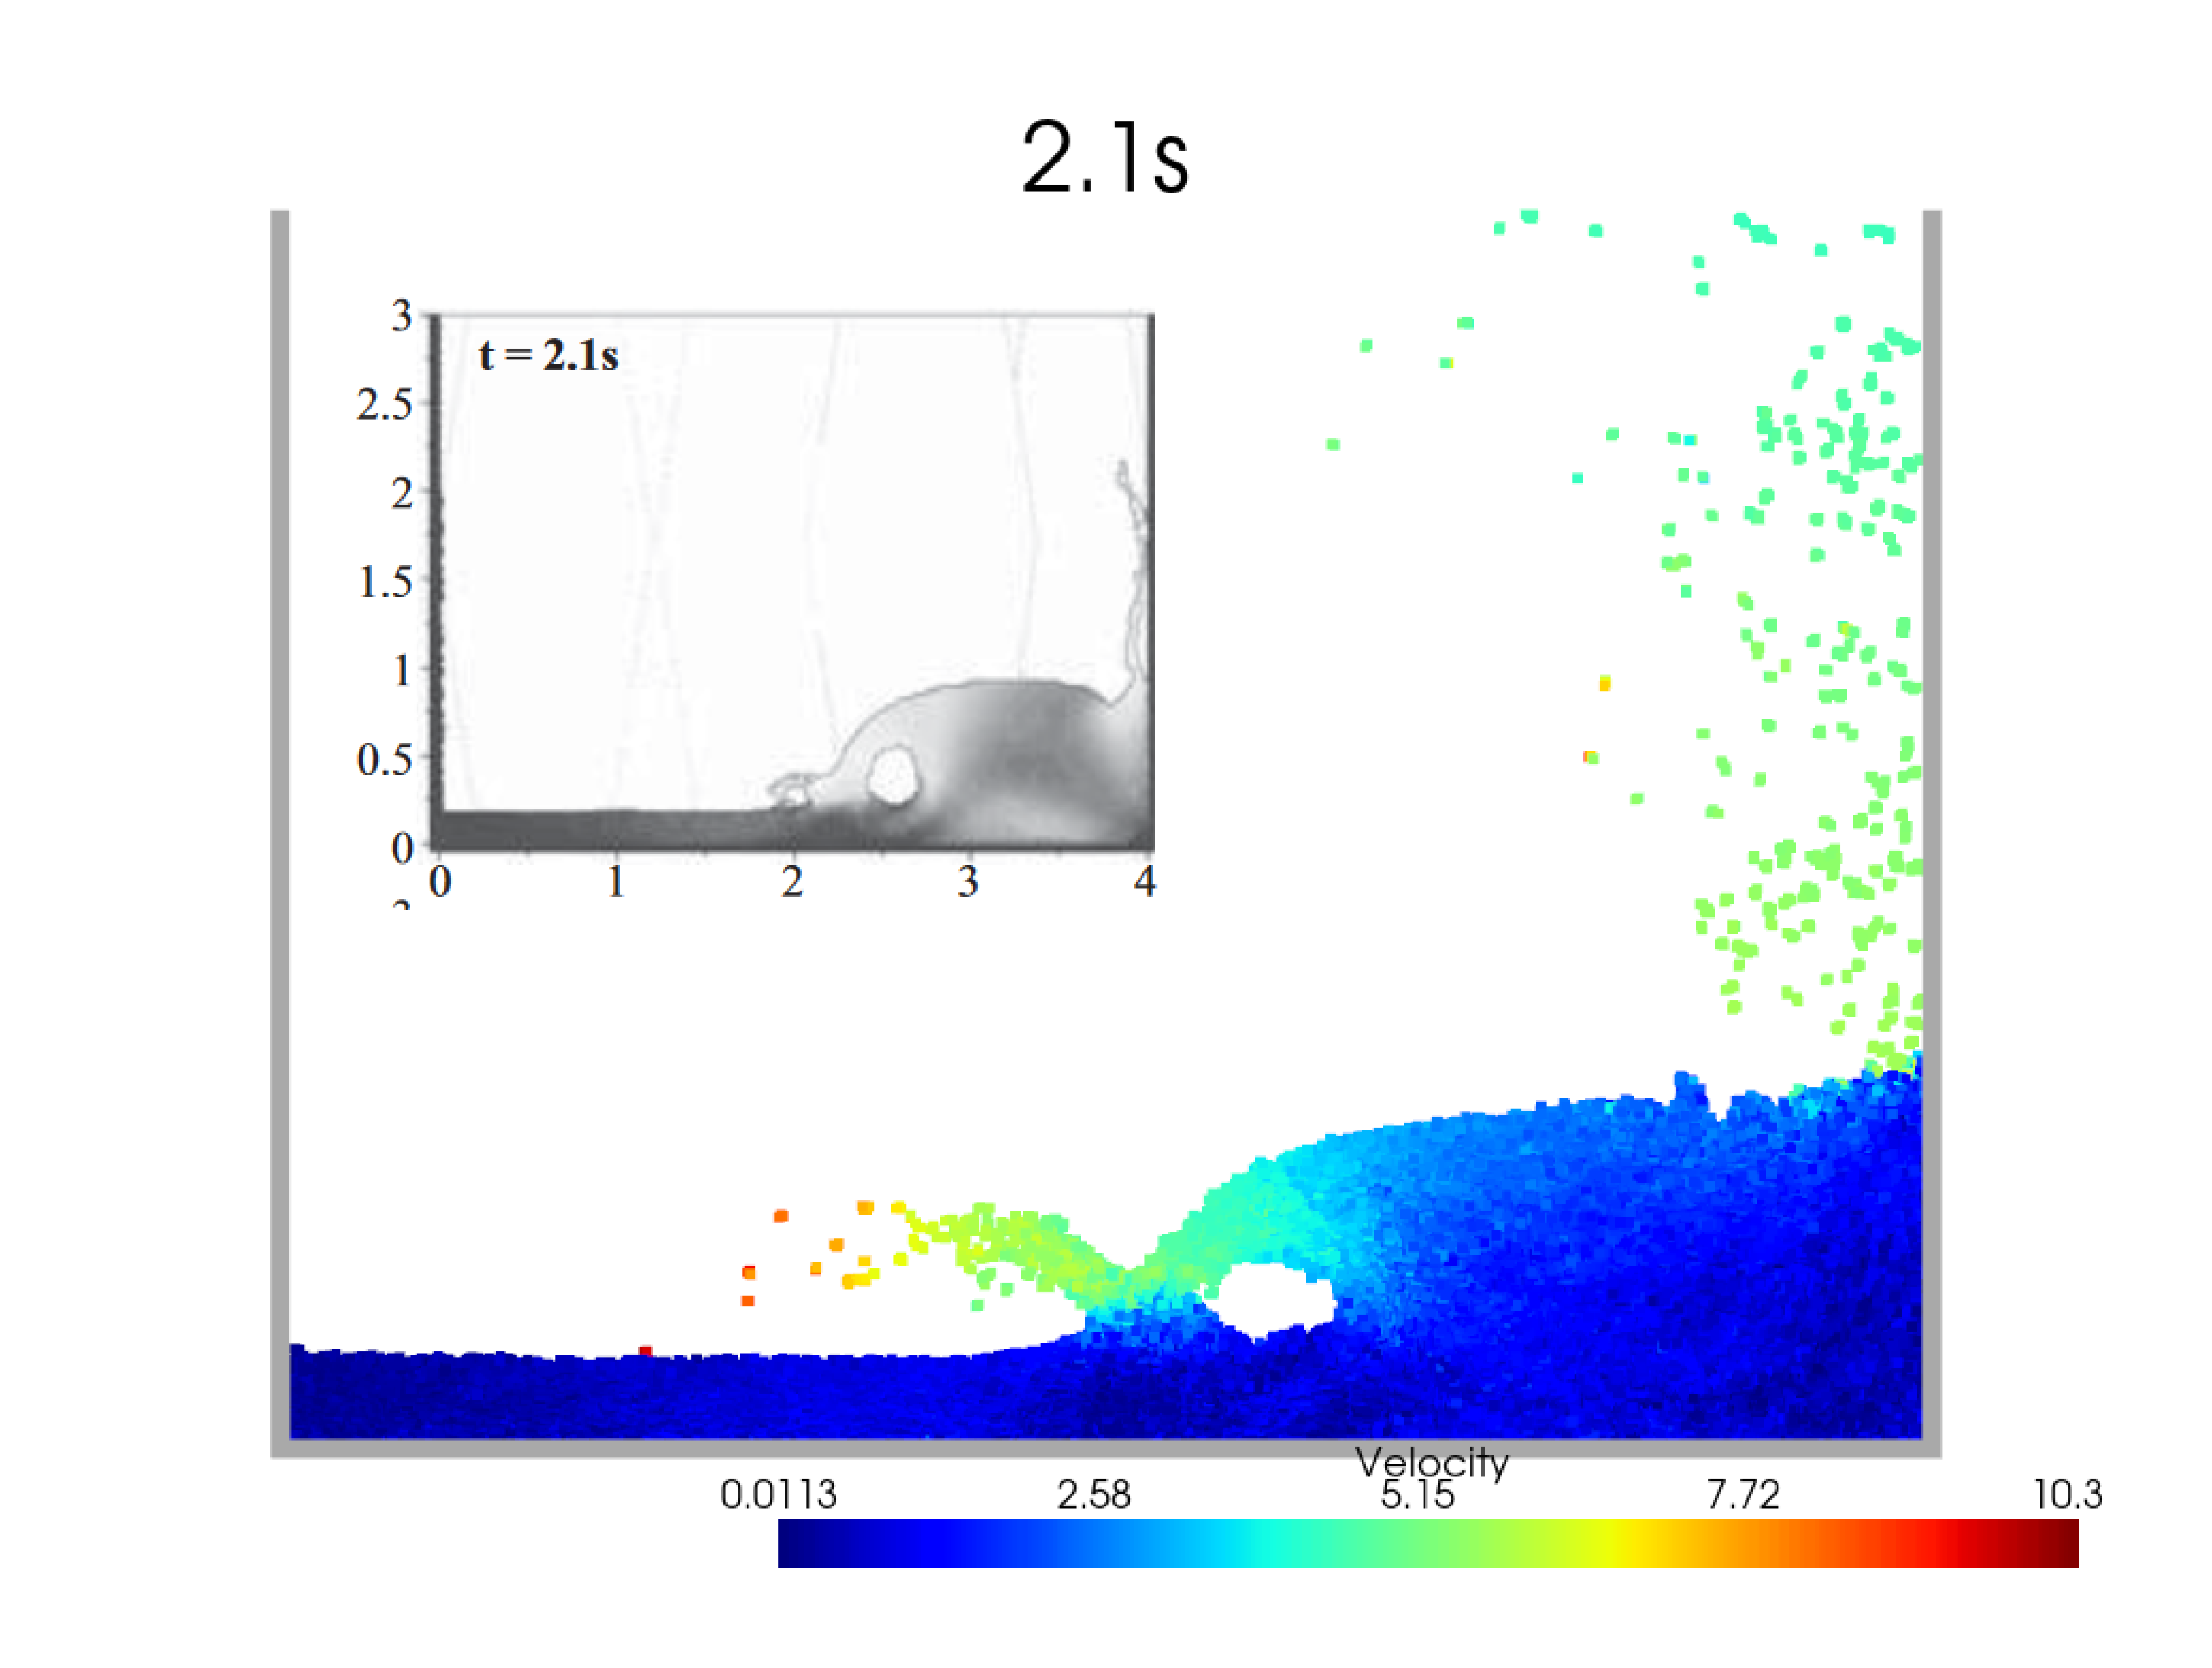
\includegraphics[width=0.9\textwidth]{images/collapse_dry21_combined.png}
    \end{figure}
\end{frame}

\begin{frame}
    \frametitle{\subsecname 2.7s}
    \begin{figure}[H]
        \centering
        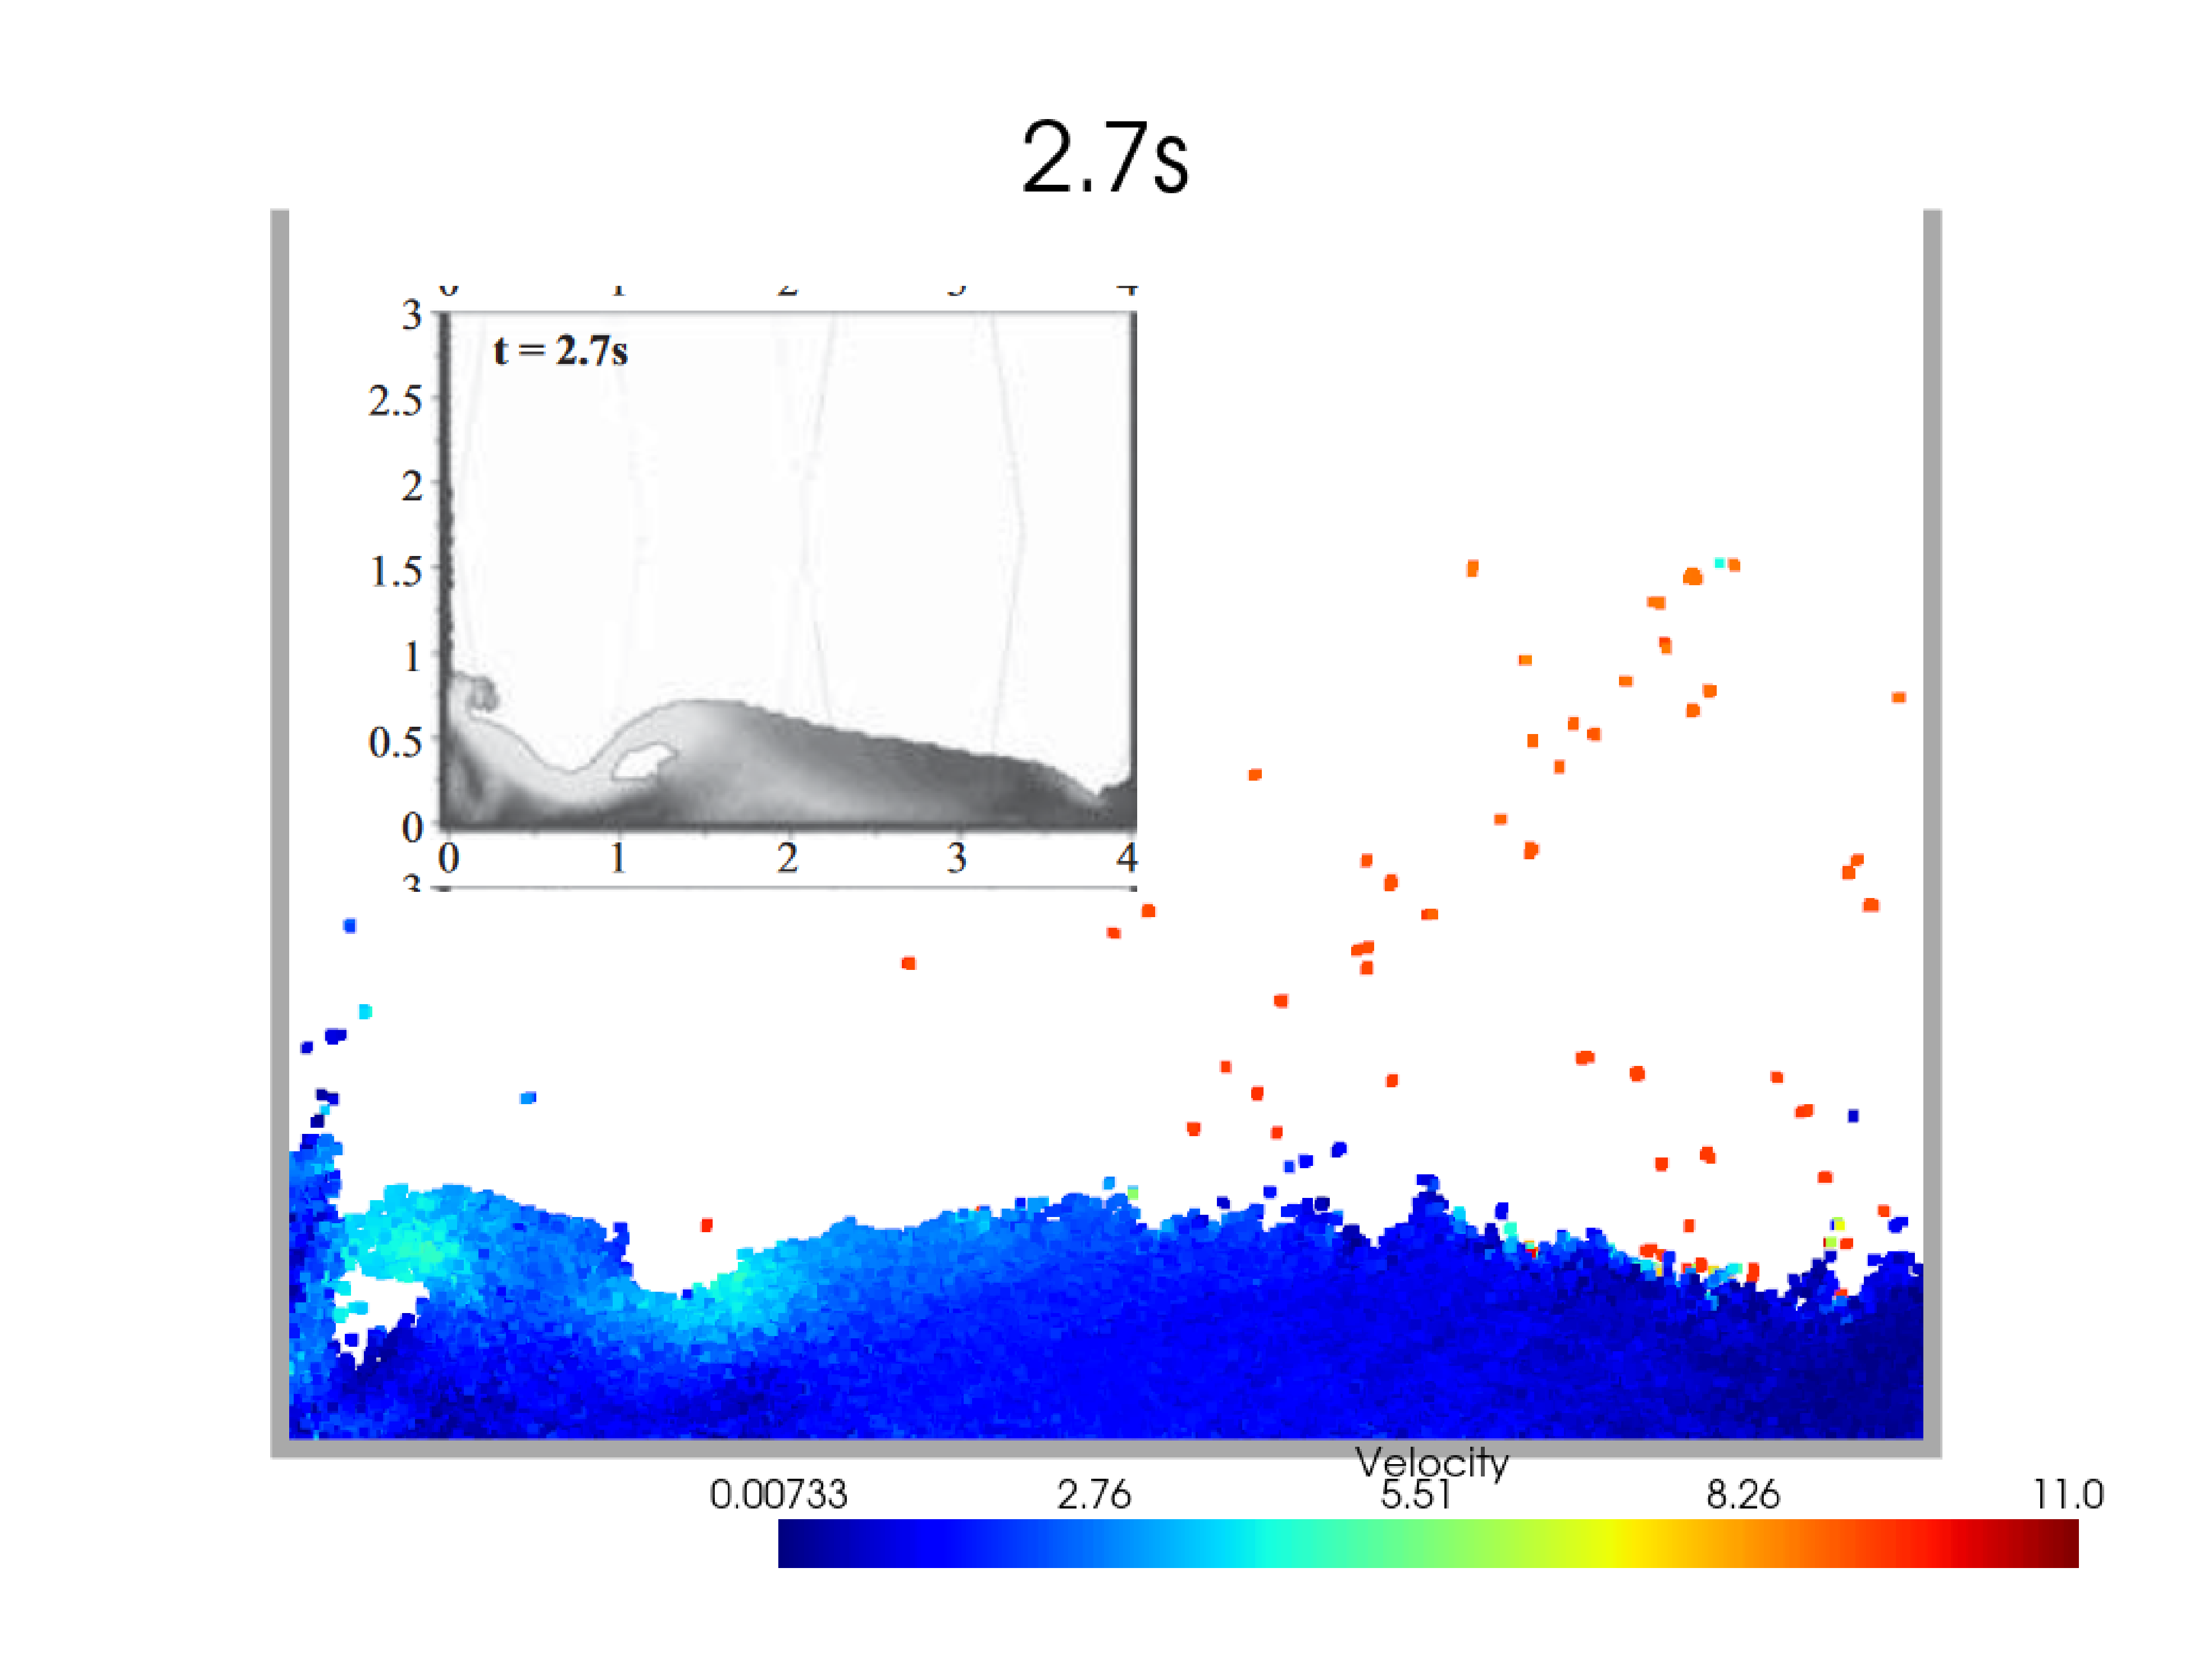
\includegraphics[width=0.9\textwidth]{images/collapse_dry27_combined.png}
    \end{figure}
\end{frame}

\begin{frame}
    \frametitle{\subsecname 2.9s}
    \begin{figure}[H]
        \centering
        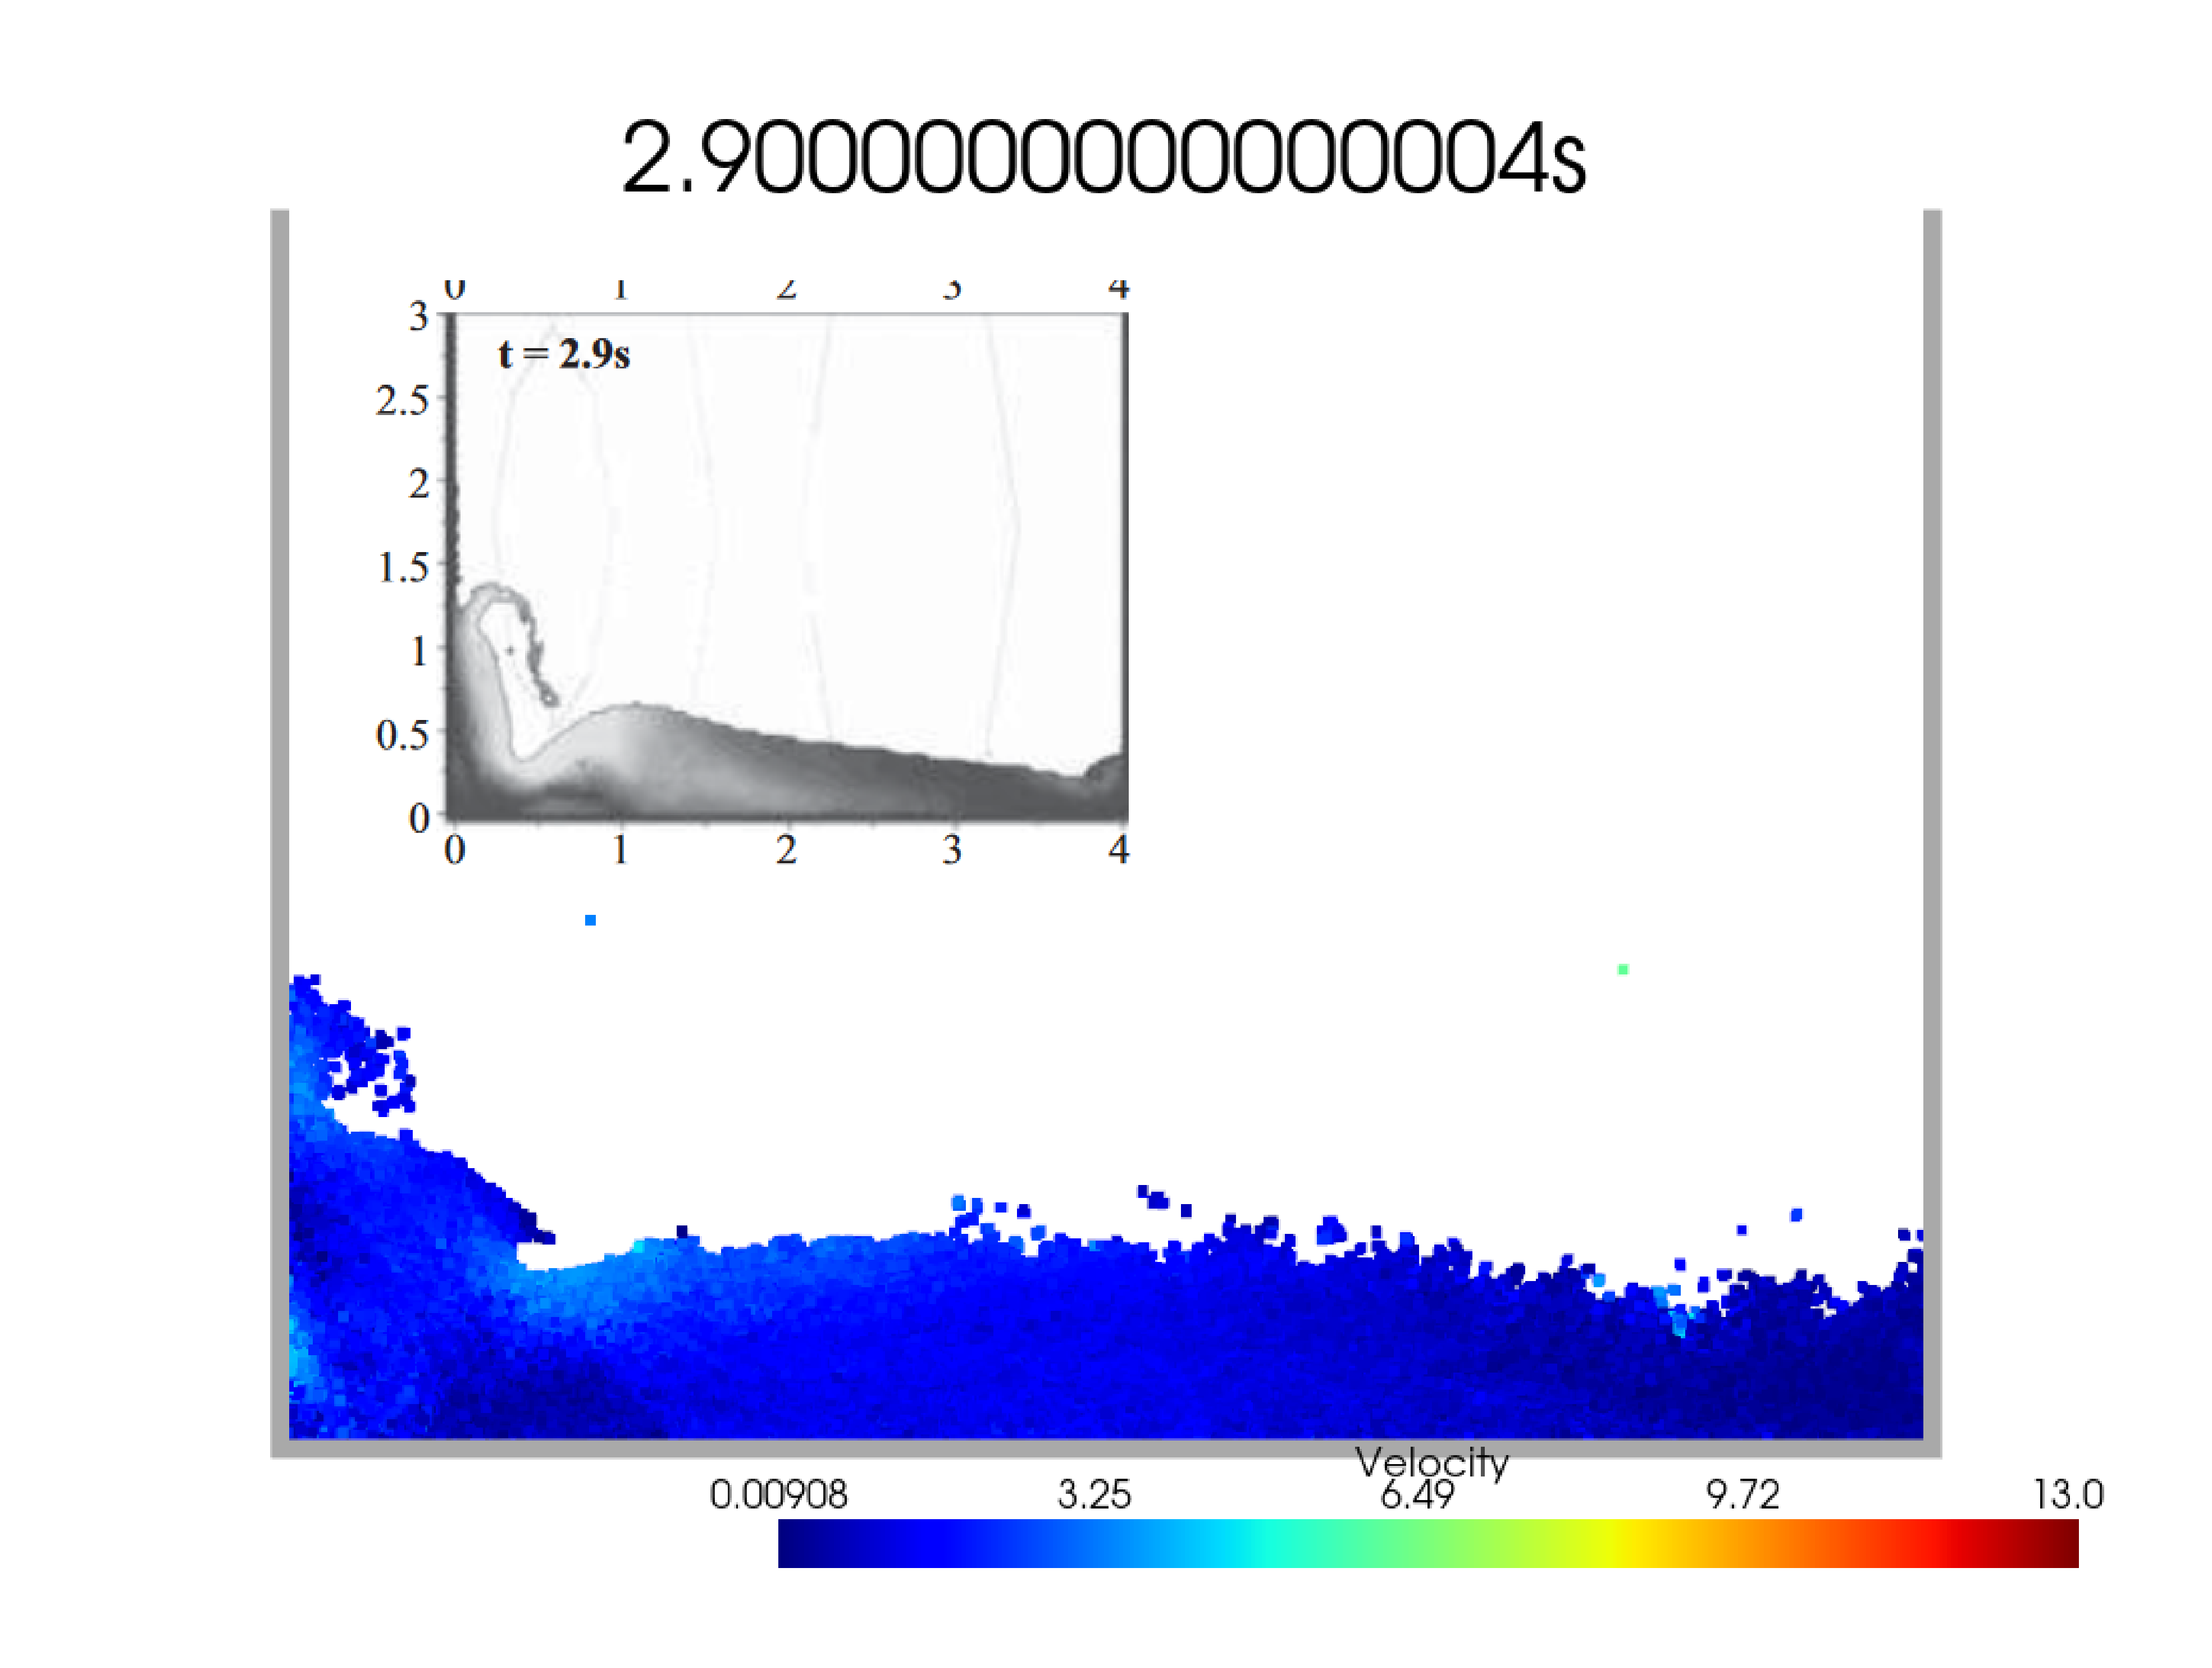
\includegraphics[width=0.9\textwidth]{images/collapse_dry29_combined.png}
    \end{figure}
\end{frame}

% \section*{参考文献}
% \begin{frame}[allowframebreaks]
% 	\frametitle{\secname}
% 	\printbibliography[heading=none]
% \end{frame}

\end{document}